%-------------------------------PPT Title-------------------------------------
\title{刘曾复教授对生理学科的贡献及其思想价值}
%-----------------------------------------------------------------------------

%----------------------------Author & Date------------------------------------
\author[]{姜~骏\inst{}
%\vskip -20pt 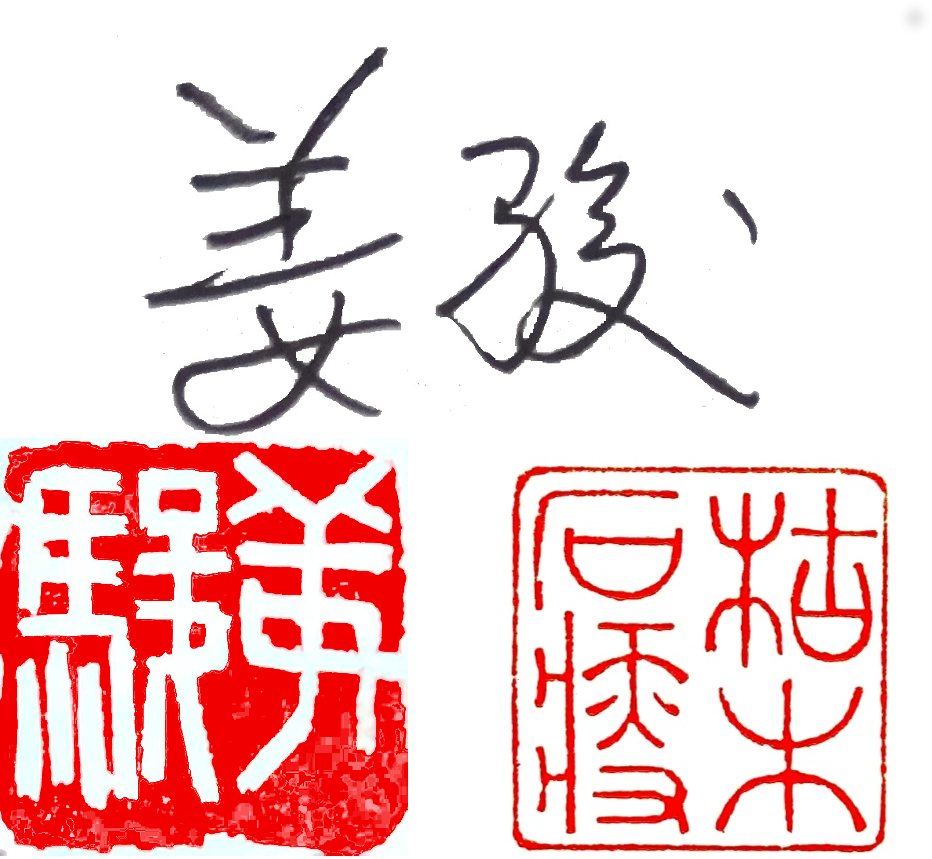
\includegraphics[scale=0.03]{Figures_Peking-Opera/signature-seal_Jiang-1.png} % 加入个人名章 
%\vskip 2pt 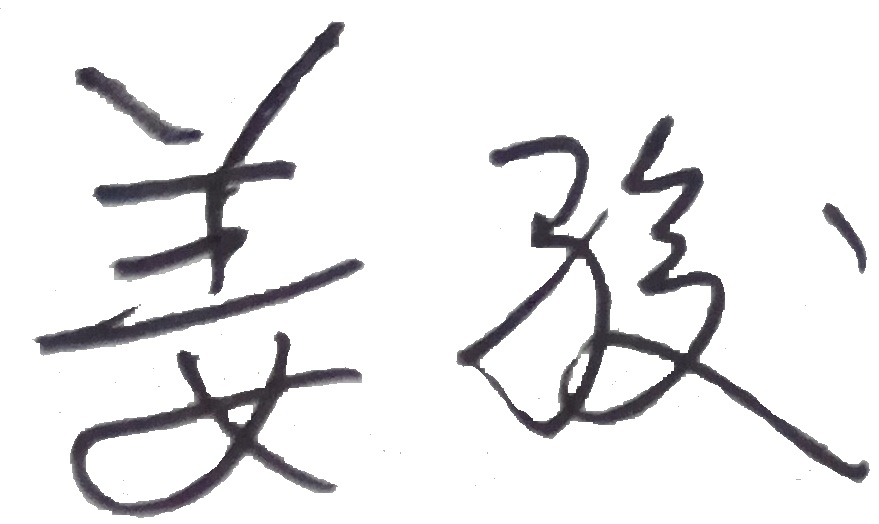
\includegraphics[scale=0.06]{Figures_Peking-Opera/signature_Jiang_new.jpg} % 加入个人签名 
%\vskip -20pt 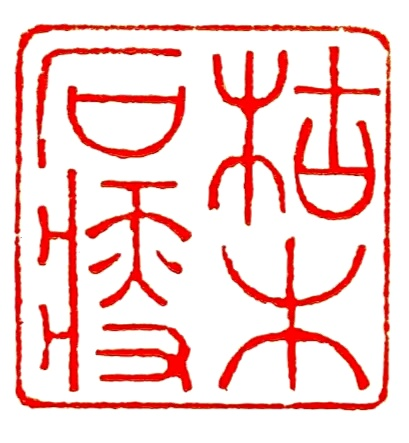
\includegraphics[scale=0.11]{Figures_Peking-Opera/seal_Jiang-2.jpg} % 加入个人闲章 
} %[]{} (optional, use only with lots of authors)
% - Give the names in the same order as the appear in the paper.
% - Use the \inst{?} command only if the authors have different
%   affiliation.
%\institute[BCC]{\inst{}%
 \vskip -30pt %北京市计算中心}
\date[\today] % (optional, should be abbreviation of conference name)
{	{\fontsize{6.2pt}{4.2pt}\selectfont{\textcolor{blue}{E-mail:~}\url{czjiangjun@yeah.cn}}}
\vskip 10 pt {\fontsize{8.2pt}{6.2pt}\selectfont{%报告地点   %清华大学\;\;物理系   
\vskip 5 pt \textrm{2024.12.19}}}
}

% - Either use conference name or its abbreviation
% - Not really information to the audience, more for people (including
%   yourself) who are reading the slides online

% This is only inserted into the PDF information catalog. Can be left
% out.
\frame[allowframebreaks]
{
	\frametitle{\fontsize{9.5pt}{5.2pt}\selectfont{\textcolor{orange}{``居今稽古''纪念刘曾复教授诞辰110周年}}}
\titlepage
}
%-----------------------------------------------------------------------------

\logo{}
%------------------------------------------------------------------------------列出全文 outline ---------------------------------------------------------------------------------
\section*{}
\frame[allowframebreaks]
{
  \frametitle{Outline}
%  \frametitle{\textcolor{mycolor}{\secname}}
  \tableofcontents%[current,currentsection,currentsubsection]
}
%在每个section之前列出全部Outline
%类似的在每个subsection之前列出全部Outline是\AtBeginSubsection[]
%\AtBeginSection[]
%{
%  \frame<handout:0>%[allowframebreaks]%讲义(handout)不显示 <handout:0> 讲义显示 <handout:1> / %beamer不显示 <beamer:0> beamer显示 <beamer:1>	
%  {
%    \frametitle{Outline}
%%全部Outline中,本部分加亮
%    \tableofcontents[current,currentsection]
%  }
%}

%------------------------------------------------------------------------------PPT main Body------------------------------------------------------------------------------------
\small
%\frame
%{
%	\frametitle{引言}
%	2000年左右,随着第一个互联网高峰的到来,戏曲艺术的传播也从传统的广播、电视媒体走向网络。
%}
\section{刘曾复教授的生理学贡献}
\frame
{
	\frametitle{学术简历}
	刘曾复教授(\textrm{1914-2012}),我国老一辈著名生理学家\\主要研究领域为普通生理学、电生理学、整合生理学
	\begin{tikzpicture}[remember picture,overlay]
	\node[xshift=-1.5cm,yshift=2.0cm] at (current page.east) {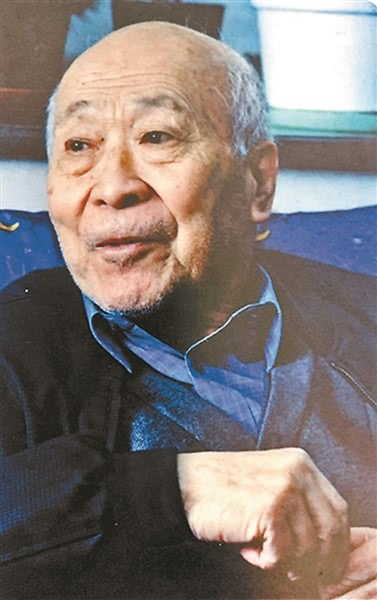
\includegraphics[height=2.2cm, width=1.70cm, viewport=0 0 377 600,clip]{/home/jun-jiang/Documents/Peking_Opera/Figures_Peking-Opera/Liu_Zengfu.jpeg}};
	\end{tikzpicture}
	\vskip 15pt
	\begin{itemize}
		\item \fontsize{9.0pt}{5.2pt}\selectfont{\textrm{1937}年,毕业于清华大学生物学系,获理学学士学位}
		\item \fontsize{9.0pt}{5.2pt}\selectfont{\textrm{1938}年\textrm{12}月起,在北平协和医学院生理学系研究实习,开始从事生命科学的研究工作}
		\item \fontsize{9.0pt}{5.2pt}\selectfont{因``太平洋战争''爆发,\textrm{1942}年初协和医学院教学及医疗工作被迫终止,到中国大学生物系担任讲师,直至抗战结束前夕}
		\item \fontsize{9.0pt}{5.2pt}\selectfont{\textrm{1945}年6月至\textrm{1960}年\textrm{6}月期间,在北京医学院(现~北京大学医学部)生理学教研室历任讲师、副教授、教授,并曾担任基础部副主任}
		\item \fontsize{9.0pt}{5.2pt}\selectfont{\textrm{1960}年,奉命由北京医学院调到北京第二医学院(现~首都医科大学),着手组建生理教研室并任主任}
		\item \fontsize{9.0pt}{5.2pt}\selectfont{\textrm{1987}年,又受学校委托,组建生物医学工程学系并担任系主任,后担任生物医学工程学院名誉主任}
	\end{itemize}
}

\frame{
	\frametitle{对我国生理学科的奠基作用:~讲义与教材}
	早在\textrm{1940}年代,刘曾复教授即已参与相关医学教材的编写
\begin{figure}[h!] 
\centering
\vspace{0.05in}
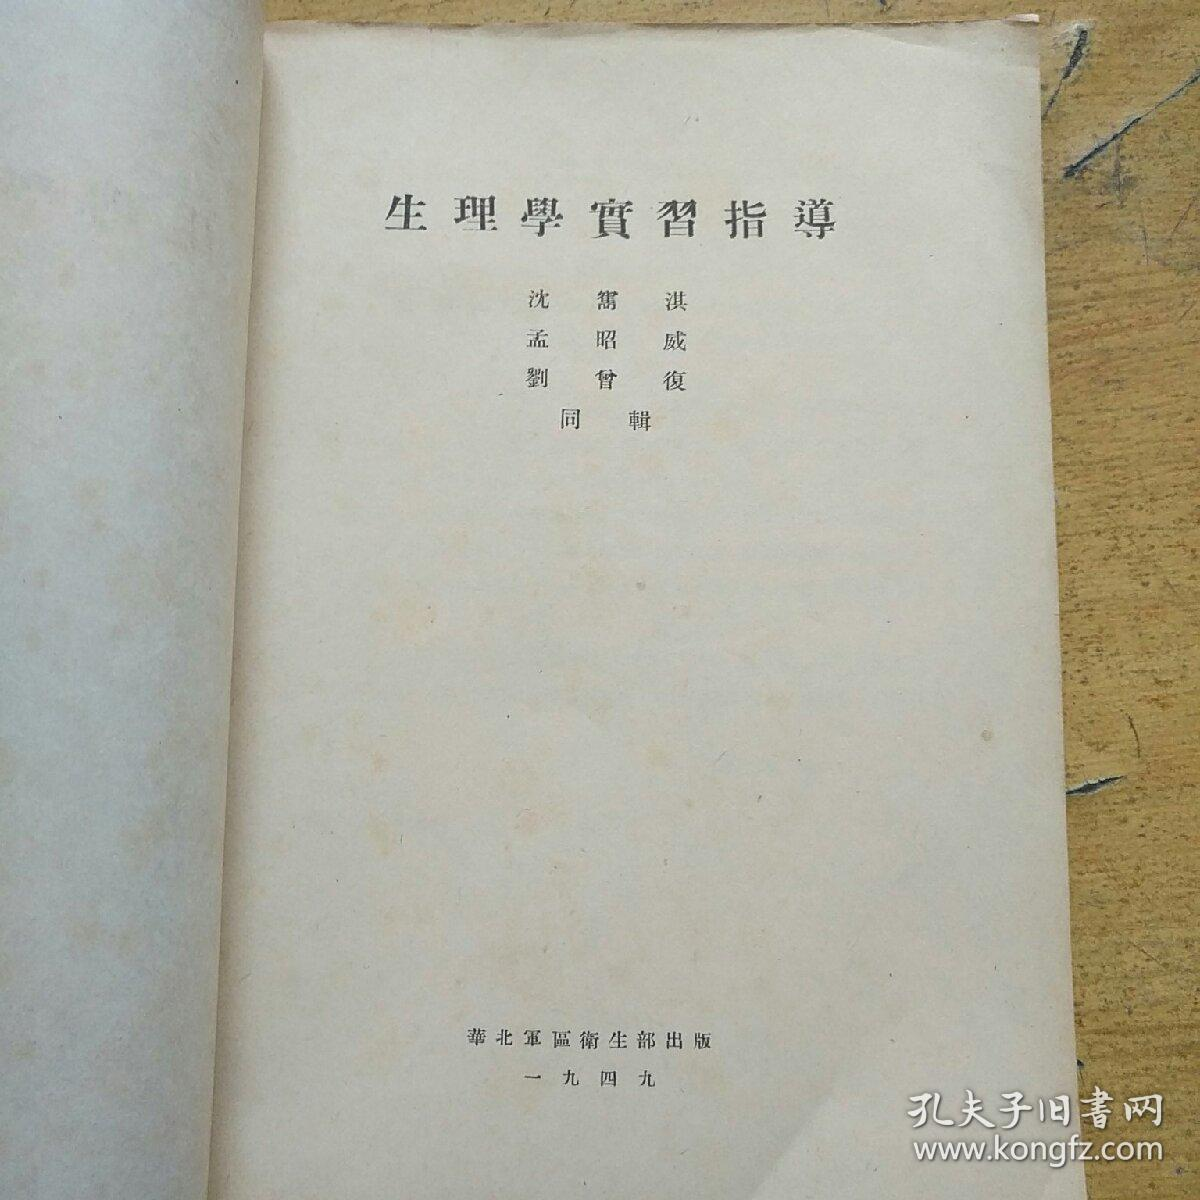
\includegraphics[height=0.55\textwidth,width=0.45\textwidth,clip]{Figures_Peking-Opera/Liu-Physiology-Pratice_2.jpg}
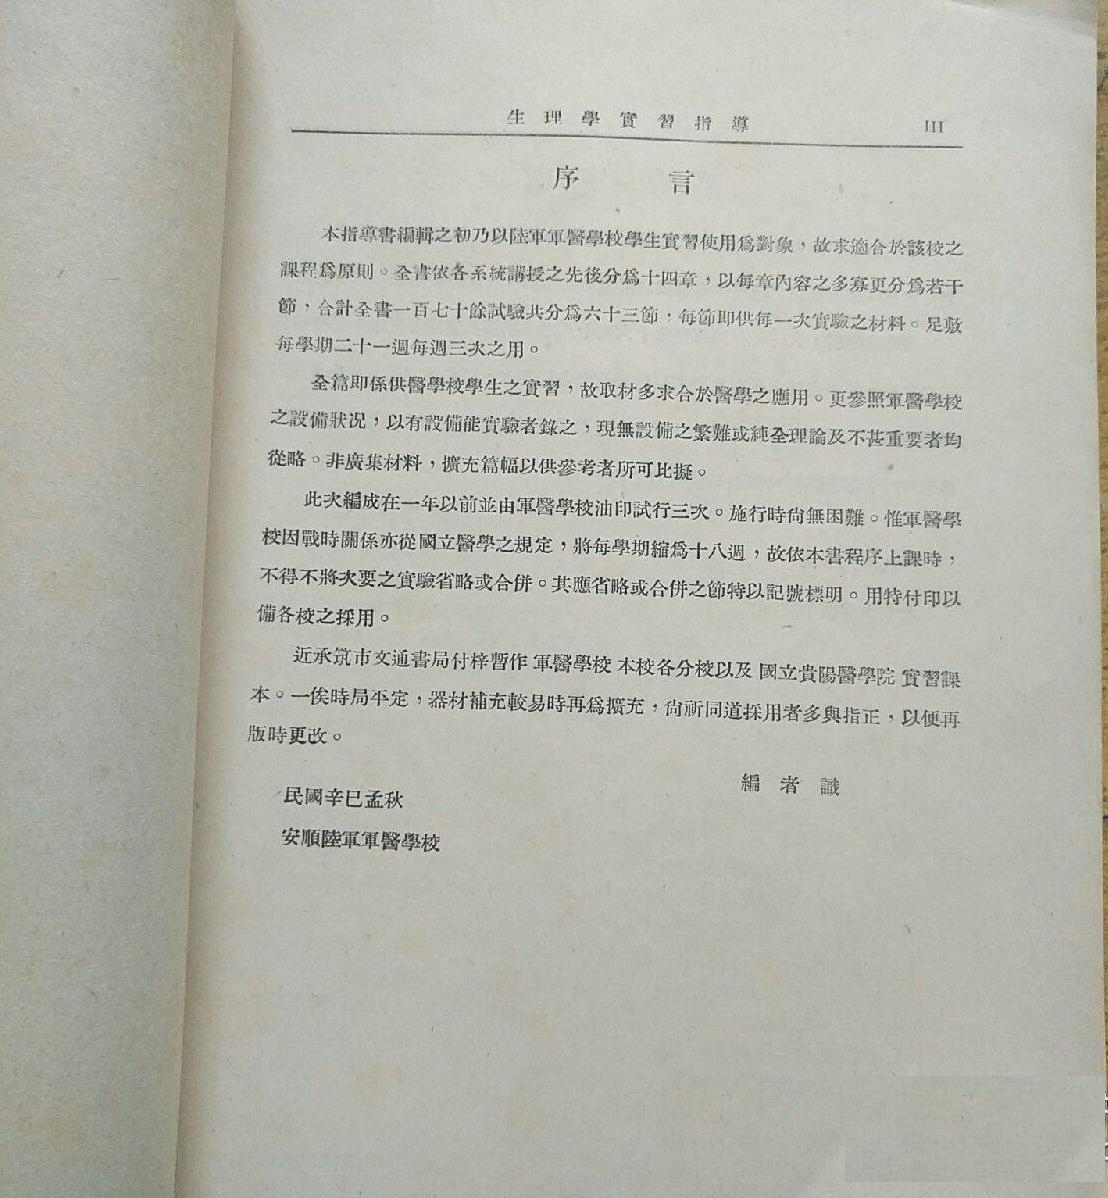
\includegraphics[height=0.55\textwidth,width=0.45\textwidth,clip]{Figures_Peking-Opera/Liu-Physiology-Pratice_3.jpg}
\label{Liu-Anatomy_and_Physiology-practice}
\end{figure}
}

\frame
{
	\frametitle{对我国生理学科的奠基作用:~讲义与教材}
	\textrm{1950-1960}年代,刘曾复教授主持编写的生理学教材,在全国中等、高等医学院校广泛使用,重印多次
\begin{figure}[h!] 
\centering
\vspace{-0.05in}
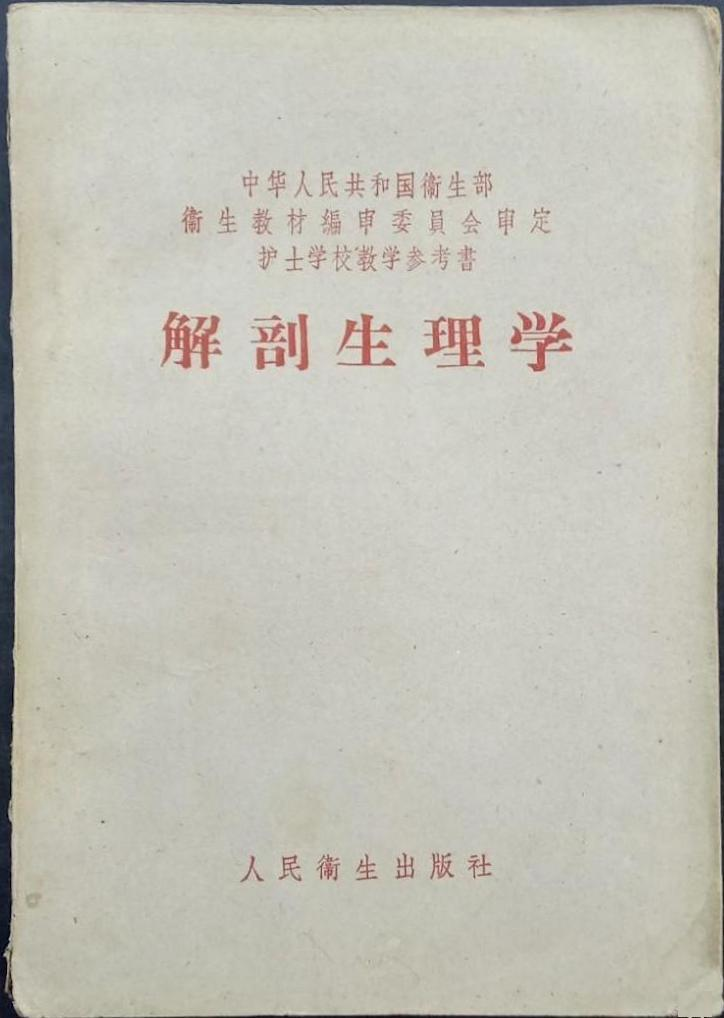
\includegraphics[height=0.45\textwidth,width=0.33\textwidth,clip]{Figures_Peking-Opera/Liu-Anatomy_and_Physiology-1.jpg}
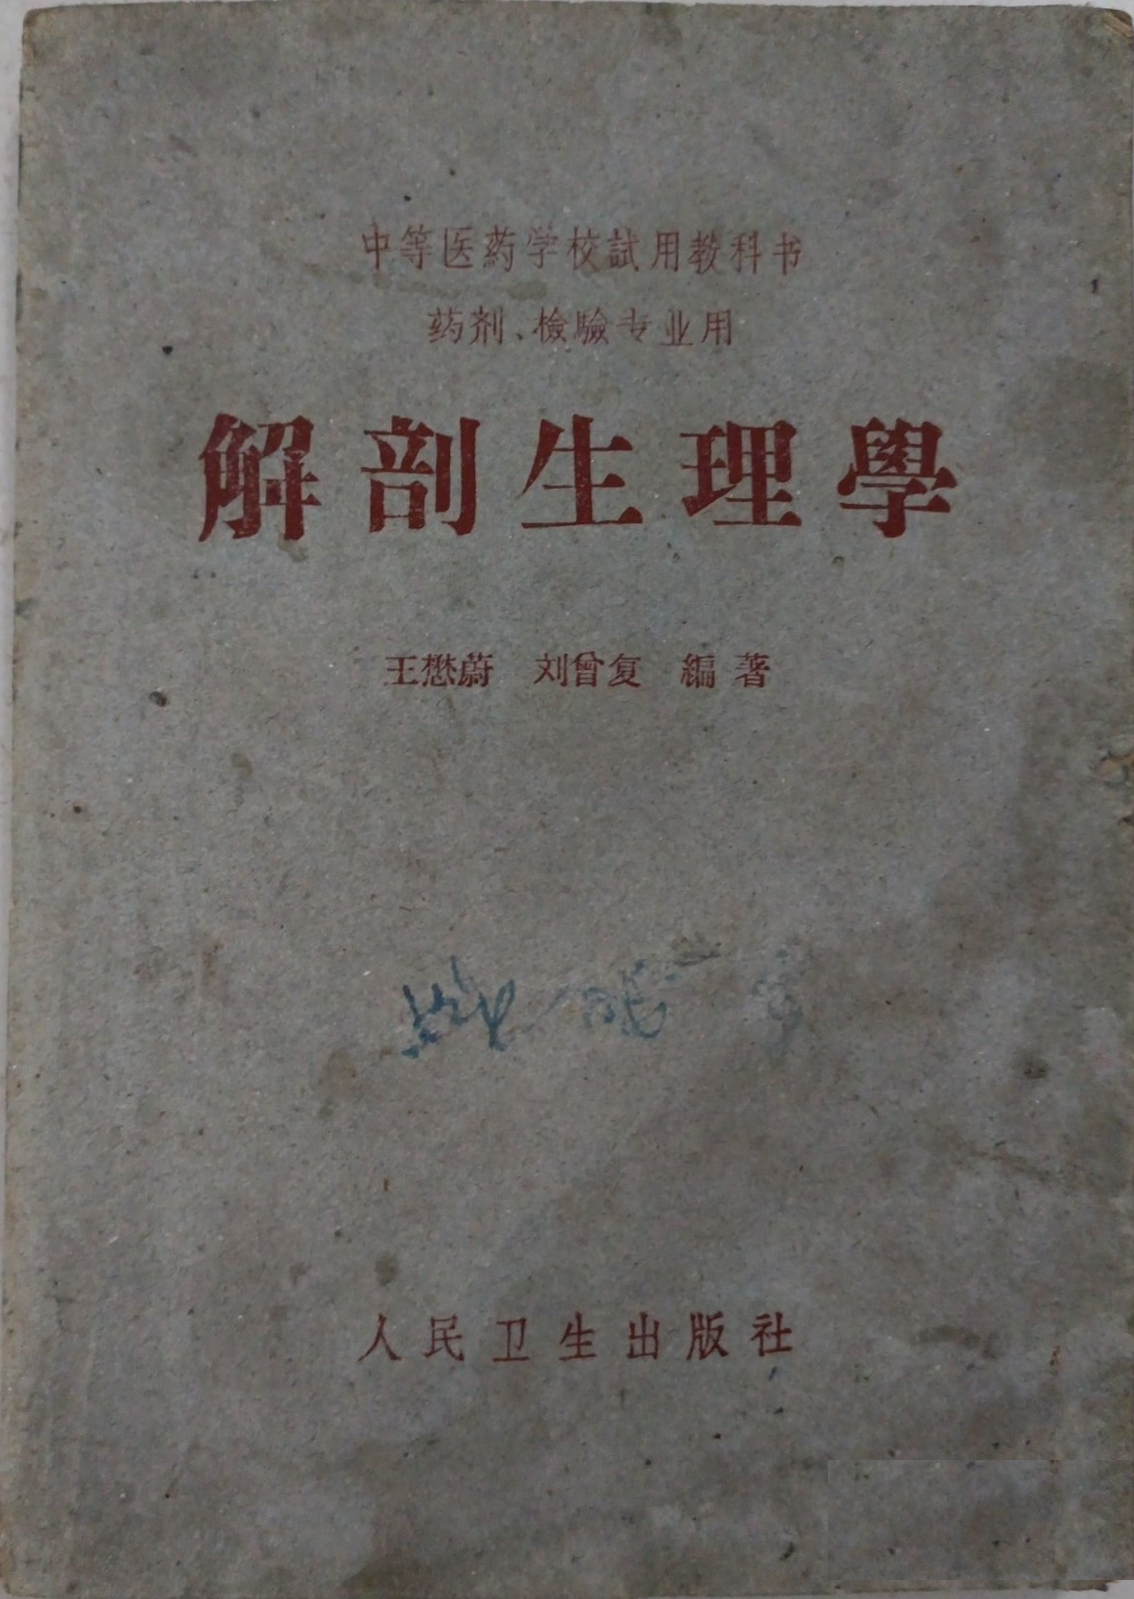
\includegraphics[height=0.45\textwidth,width=0.33\textwidth,clip]{Figures_Peking-Opera/Liu-Anatomy_and_Physiology-3.jpg}
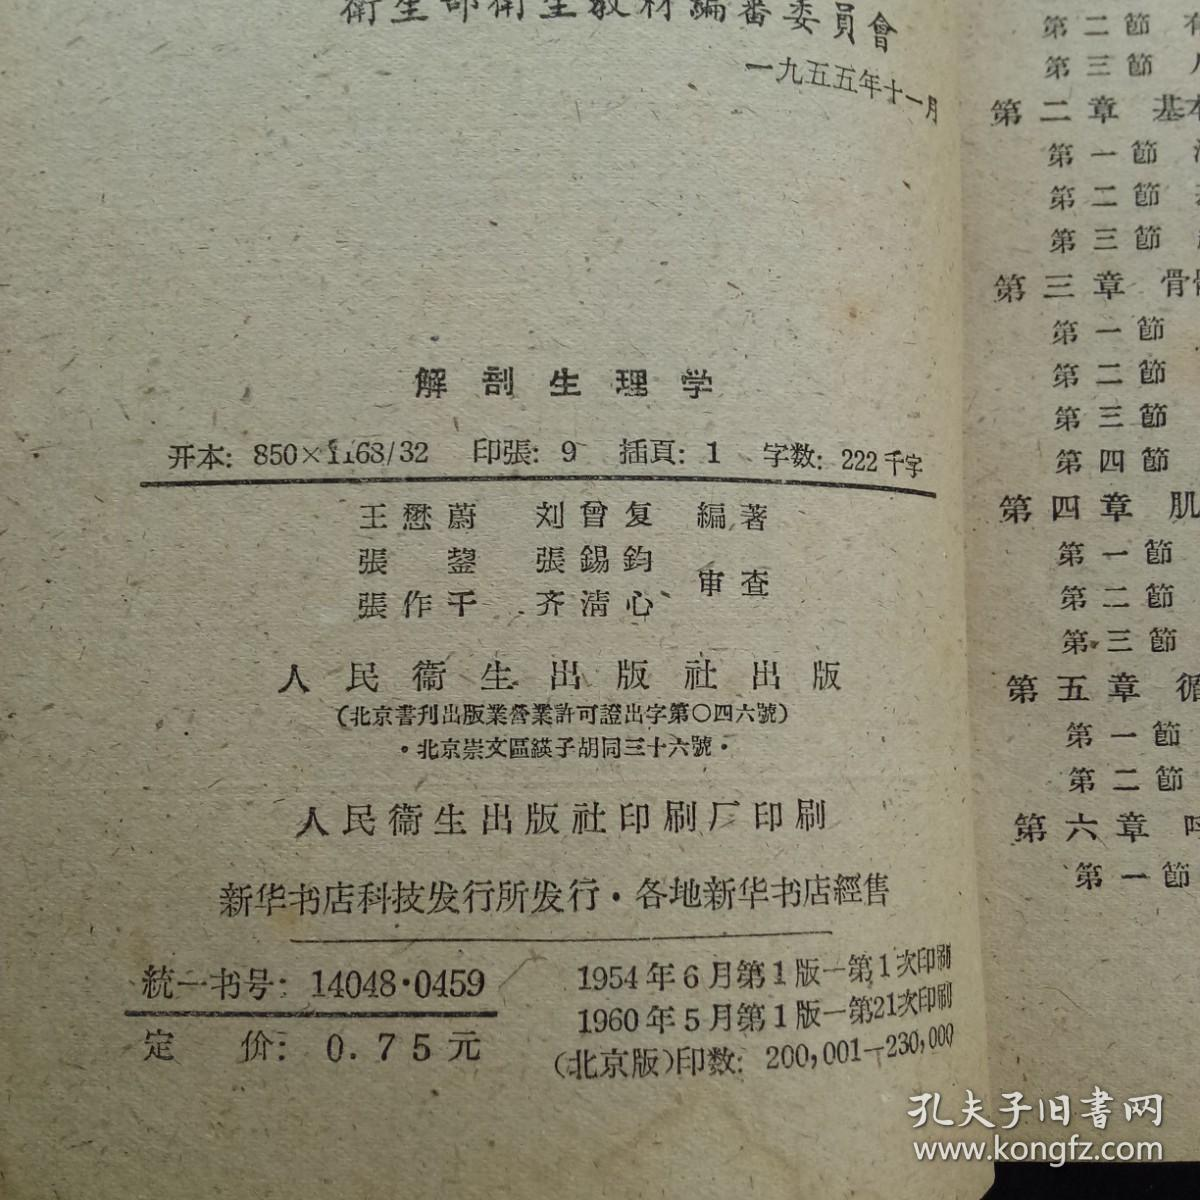
\includegraphics[height=0.18\textwidth,width=0.40\textwidth,viewport=0 70 1071 630,clip]{Figures_Peking-Opera/Liu-Anatomy_and_Physiology-2.jpg}
\label{Liu-Anatomy_and_Physiology-middle}
\end{figure}
}

\frame
{
	\frametitle{对我国生理学科的奠基作用:~讲义与教材}
\begin{figure}[h!] 
\centering
\vspace{-0.05in}
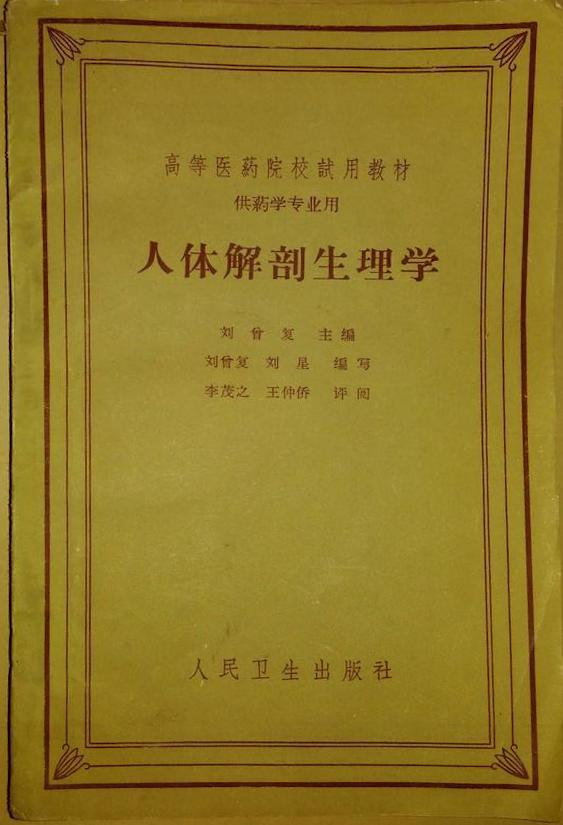
\includegraphics[height=0.48\textwidth,width=0.35\textwidth,clip]{Figures_Peking-Opera/Liu-Anatomy_and_Physiology-5.jpg}
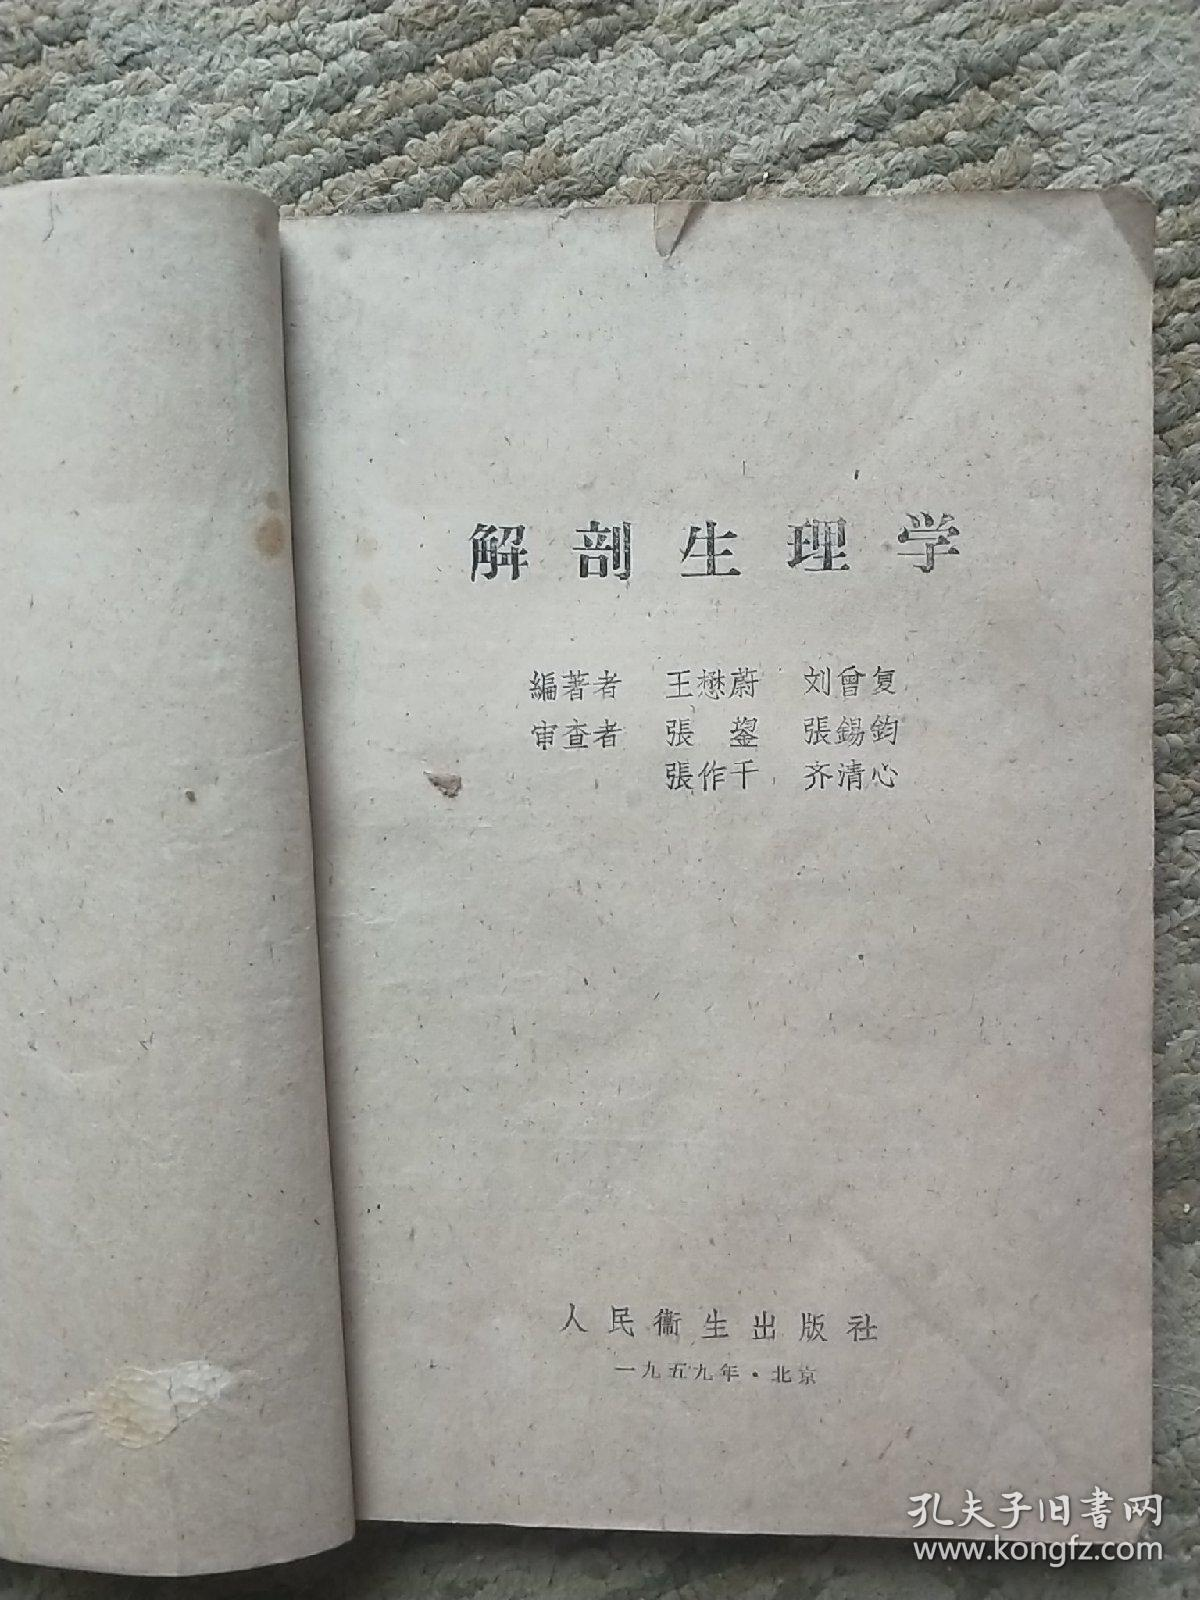
\includegraphics[height=0.48\textwidth,width=0.35\textwidth,clip]{Figures_Peking-Opera/Liu-Anatomy_and_Physiology-7.jpg}
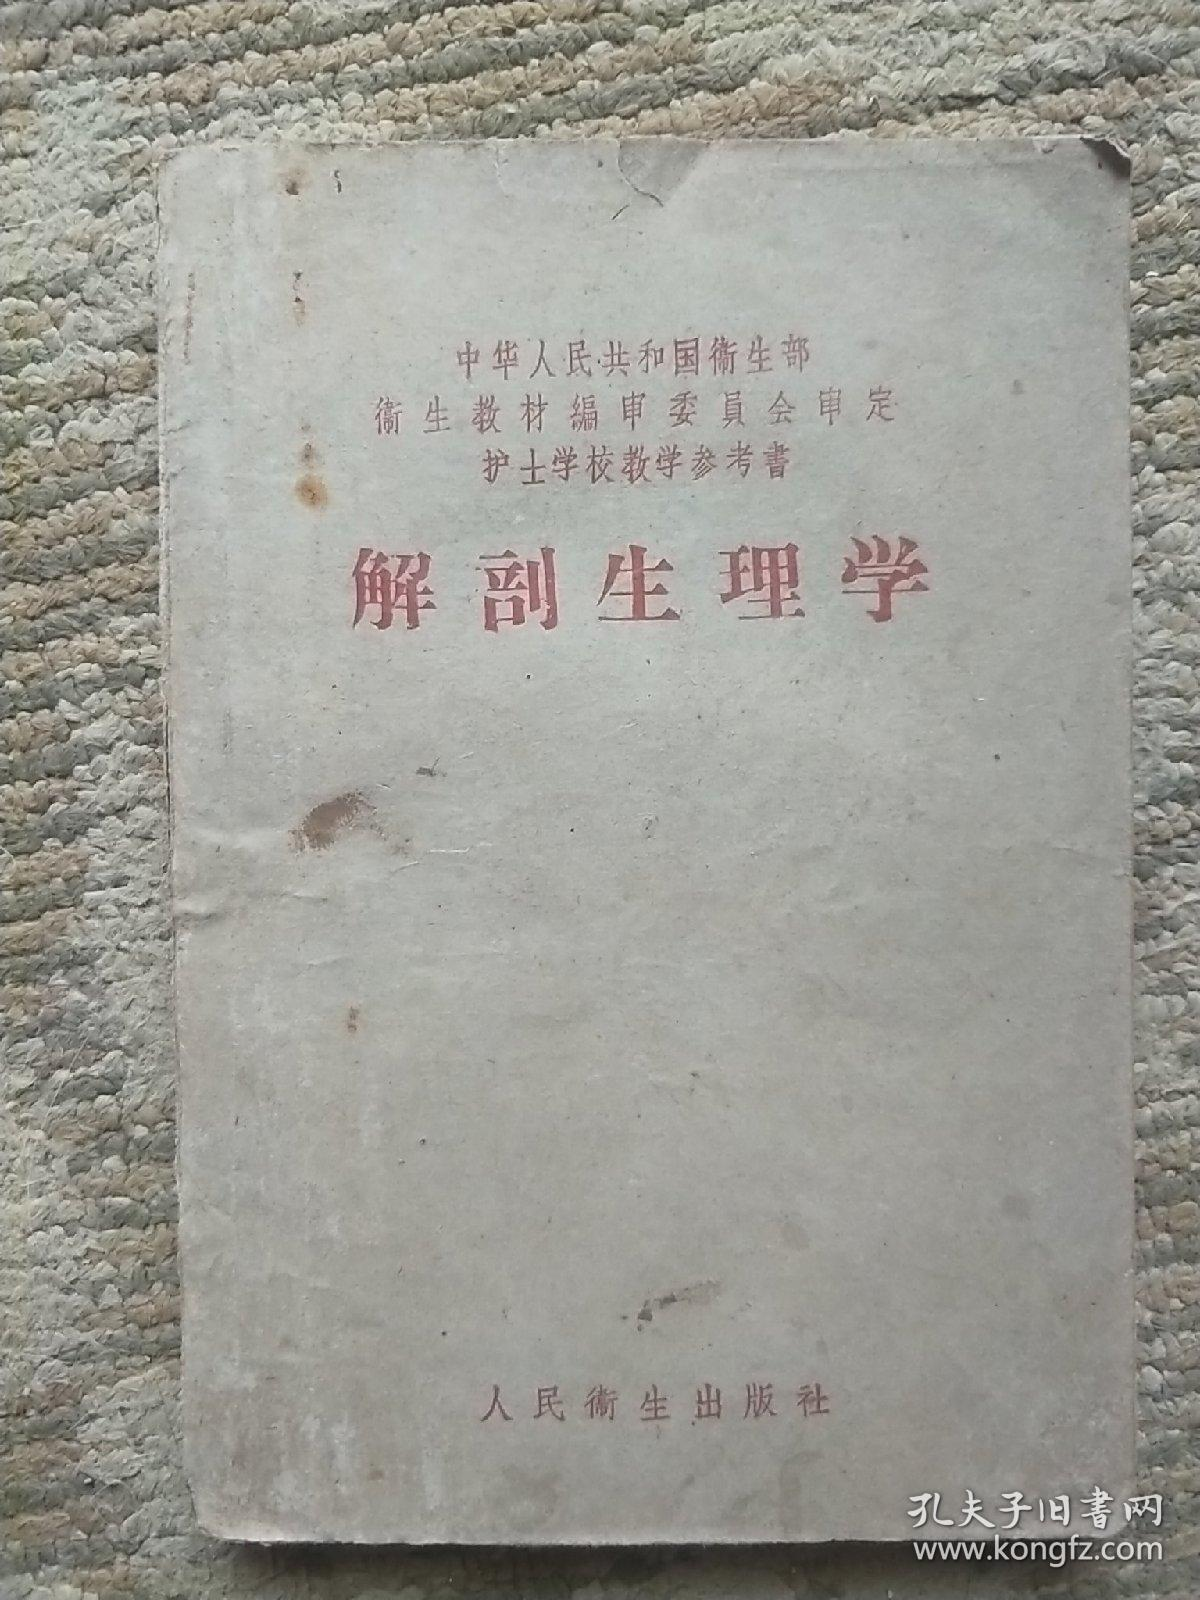
\includegraphics[height=0.22\textwidth,width=0.45\textwidth,viewport=0 70 548 330,clip]{Figures_Peking-Opera/Liu-Anatomy_and_Physiology-6.jpg}
\label{Liu-Anatomy_and_Physiology-college}
\end{figure}
}

\frame
{
	\frametitle{生理学研究的学术成果:~代表论文}
	刘曾复教授毕生的研究经历
	\begin{itemize}
		\item 普通生理学:~垂体活动、代谢与消化的神经与体液调节\\
			{\fontsize{6.2pt}{4.2pt}\selectfont{\textrm{Hsi-Chun Chang, \underline{Tseng-Fu Liu} and Shih-Yi, Pan, \textcolor{blue}{Influence of Testisterone Propionate On the Gonadotropic Potency of The Anterior Pituitary}, \textit{Chinese Journal of Physiology}, \textbf{16}(1), 57, 1941}}}
		\item 电生理学\\
			{\fontsize{6.2pt}{4.2pt}\selectfont{\textrm{陈兰生、\underline{刘曾复}、沈寯淇, \textcolor{blue}{蟾蜍中枢神经系统的抑制过程和脑电图的关系}, \textit{生理学报}, \textbf{24}(1), 47, 1960}}}\\
		\item 神经系统的整合作用研究与控制论\\ 
			{\fontsize{6.2pt}{4.2pt}\selectfont{\textrm{王雨若、张英才、赵紫东、\underline{刘曾复},\textcolor{blue}{刺激迷走神经对皮层诱发性下颌运动的抑制作用},\textit{生理学报},\textbf{26}(3), 251, 1963}}}\\
			{\fontsize{6.2pt}{4.2pt}\selectfont{\textrm{李效义、刘北英、张淑华、张英才、\underline{刘曾复},\textcolor{blue}{氨刺激兔鼻粘膜引起心血管反应的神经机制分析},\textit{首都医科大学学报},\textbf{8}(3),163, 1987}}}\\
			{\fontsize{6.2pt}{4.2pt}\selectfont{\textrm{\underline{刘曾复}、丁延衸、赵以炳, \textcolor{blue}{控制理论与生理控制系统},\textit{生理科学进展},\textbf{9}(2),97, 1978}}}
	\end{itemize}
}

\frame
{
	\frametitle{生理学研究的学术成果:~专著}
	进入到\textrm{1980}年代,随着生理科研活动的重新有序开展,刘曾复教授编写了关于神经生理学研究的专著,发表了普及生理学基础知识的系列论文。此外,特别重视数学作为逻辑推演工具在生物学研究中的运用
\begin{figure}[h!] 
\centering
\vspace{-0.05in}
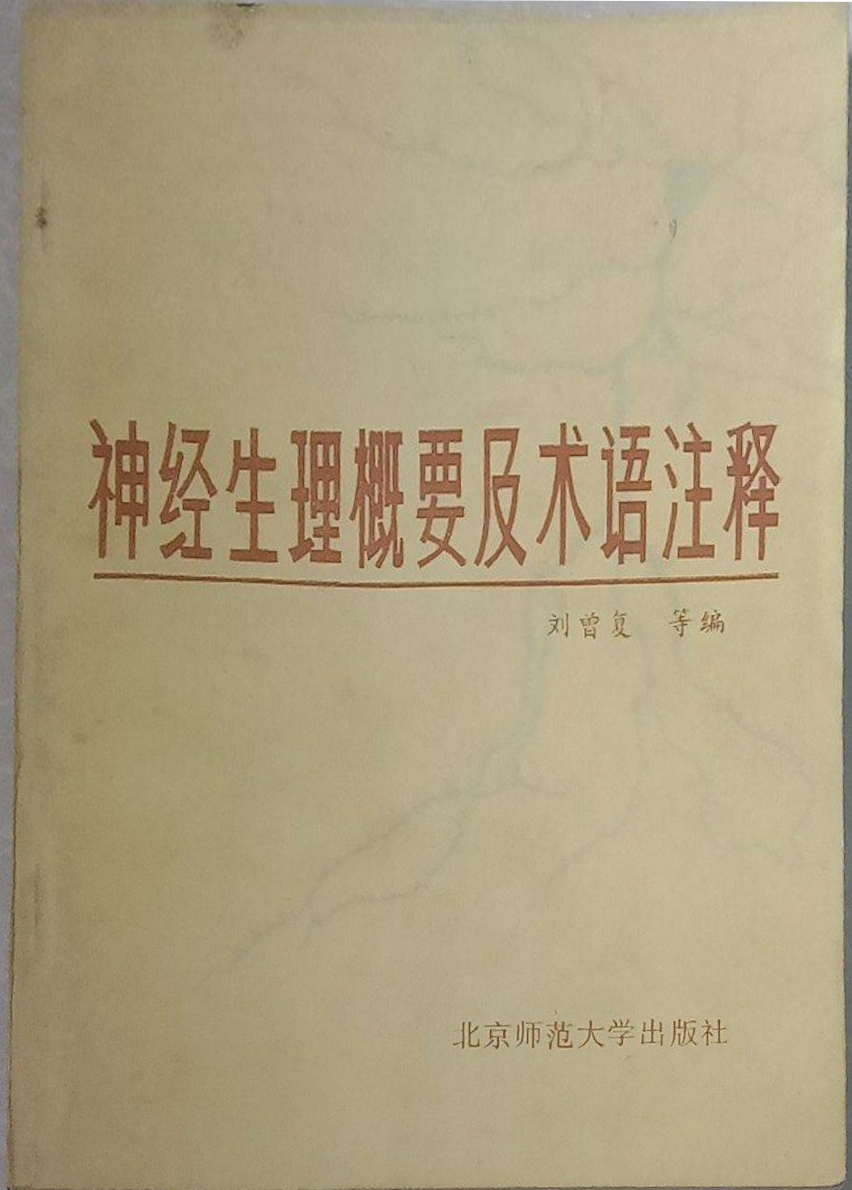
\includegraphics[height=0.52\textwidth,width=0.38\textwidth,clip]{Figures_Peking-Opera/Liu-Neurophysiology-1.jpg}
%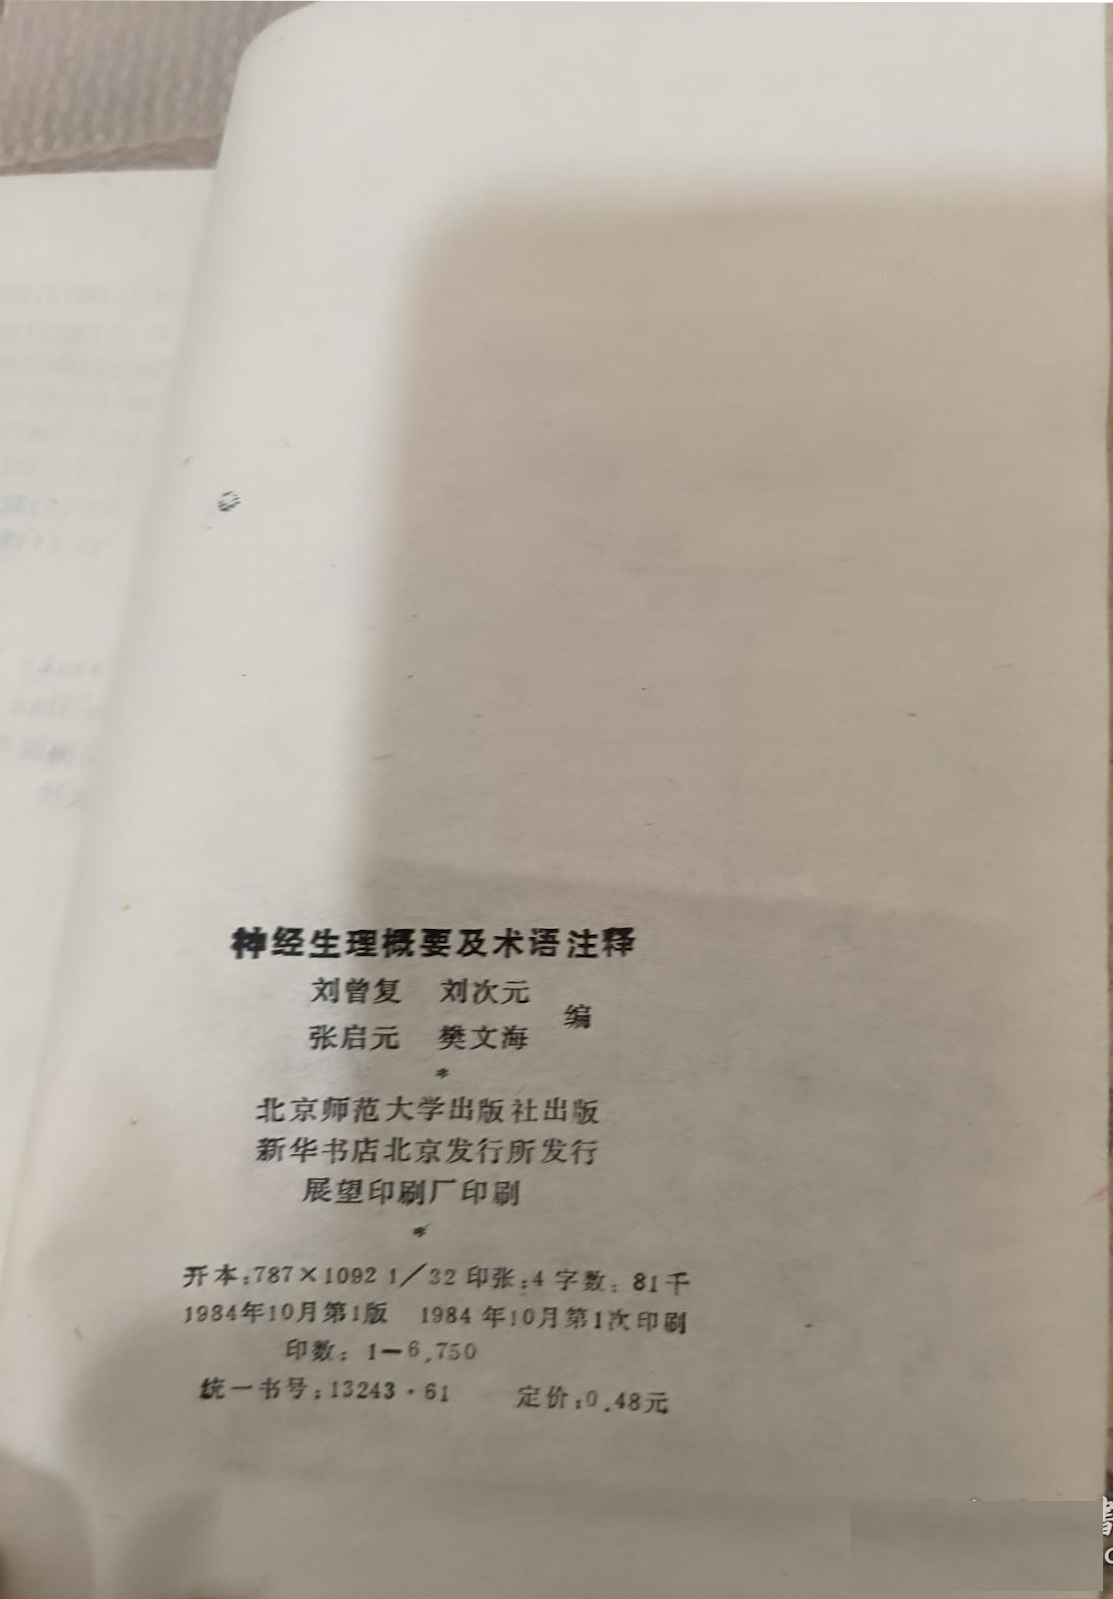
\includegraphics[height=0.48\textwidth,width=0.35\textwidth,clip]{Figures_Peking-Opera/Liu-Neurophysiology-2.jpg}
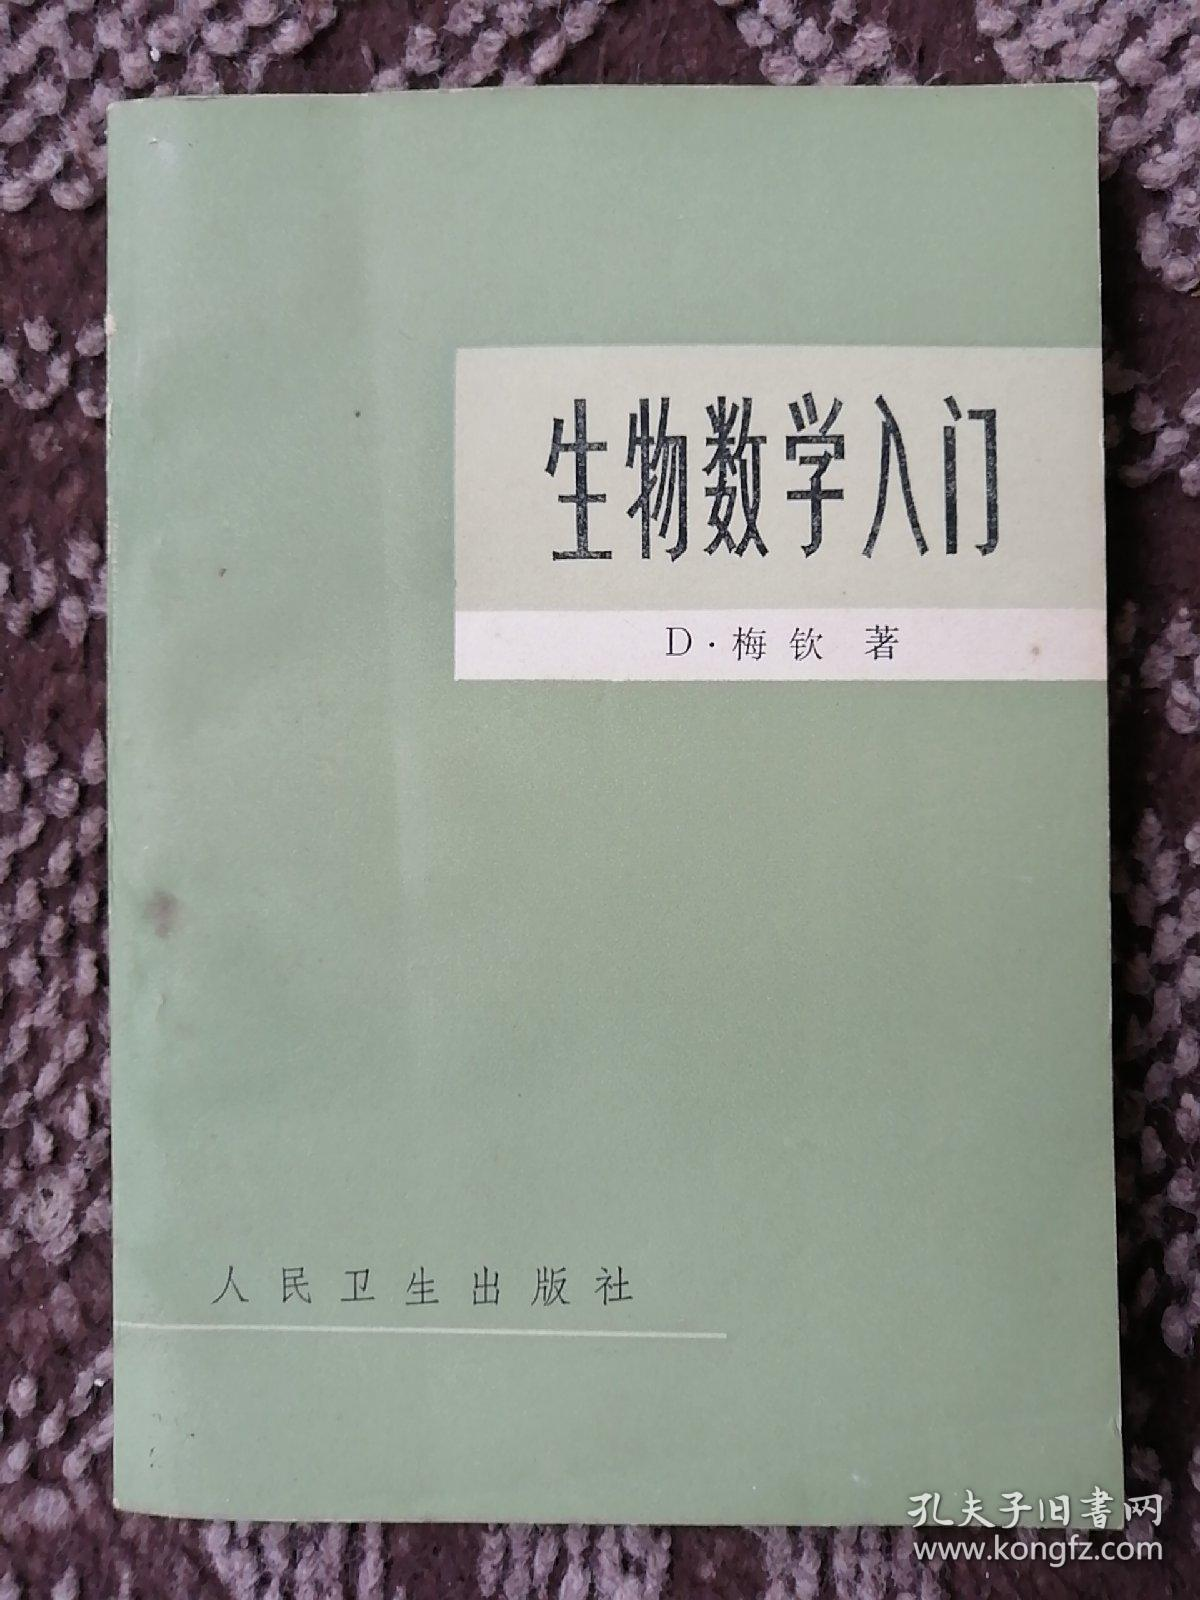
\includegraphics[height=0.52\textwidth,width=0.38\textwidth,clip]{Figures_Peking-Opera/Liu-Mathematic.jpg}
\label{Liu-Anatomy_and_Physiology-college}
\end{figure}
}

\frame
{
	\frametitle{对生理学研究的展望和建议}
	{\fontsize{6.2pt}{4.2pt}\selectfont{\textrm{\underline{刘曾复}, \textcolor{blue}{生理学研究方法的回顾与前瞻——学说、实验和计算机在生理学研究中的作用},\textit{生物学通报},\textbf{1},21, 1985}}}
\begin{figure}[h!] 
\centering
\vspace{-0.08in}
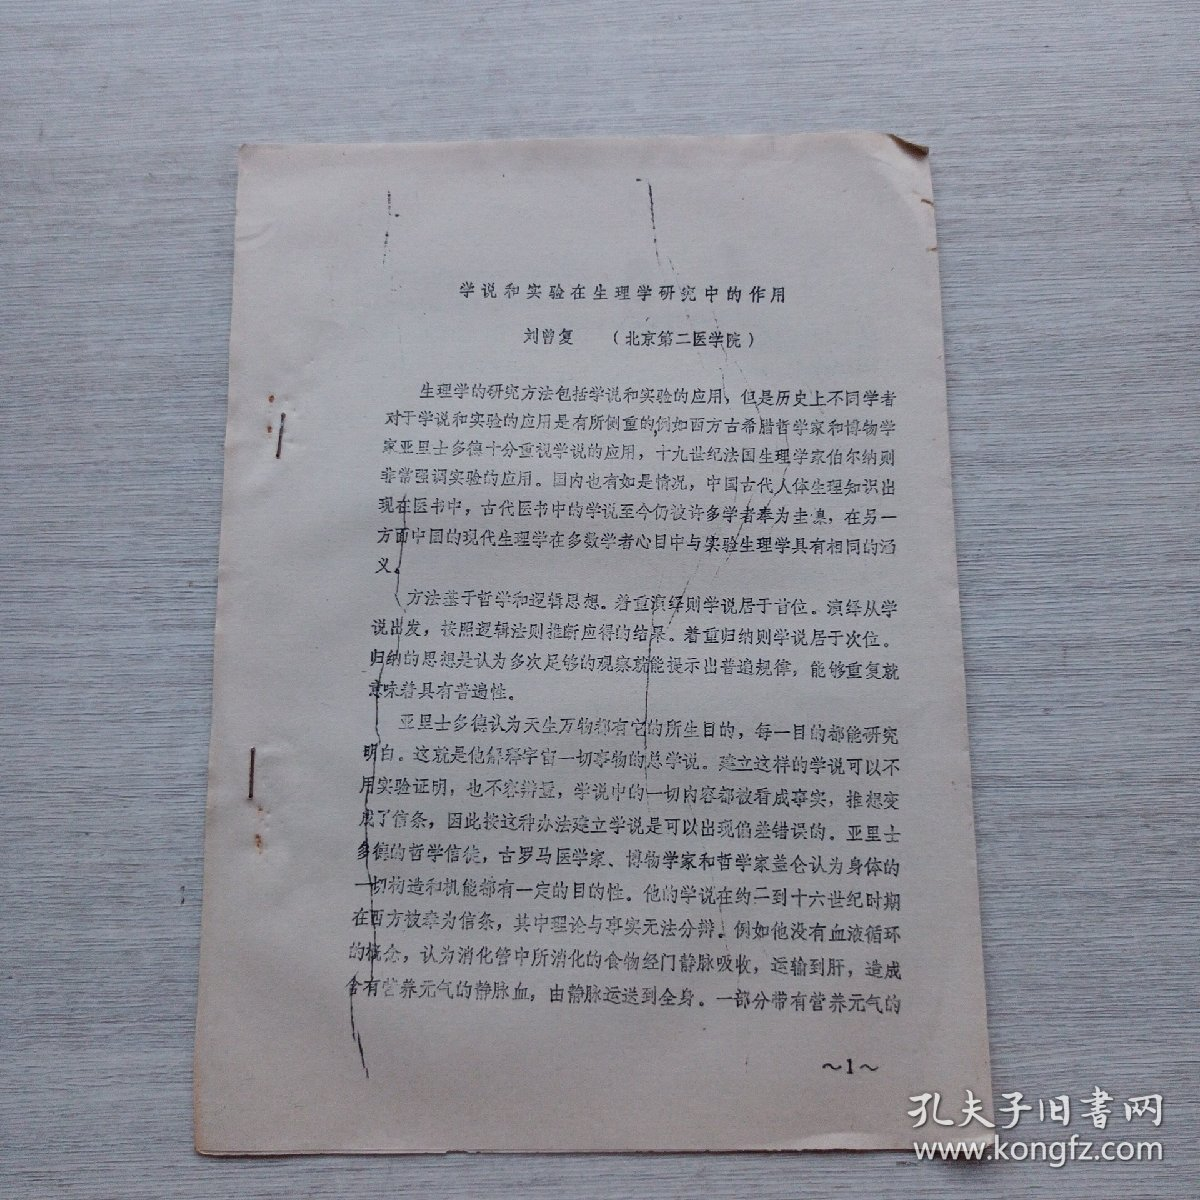
\includegraphics[height=0.60\textwidth,width=0.48\textwidth,clip]{Figures_Peking-Opera/Liu-Paper.jpg}
\includegraphics[height=0.40\textwidth,width=0.40\textwidth,clip]{/home/jun-jiang/Documents/Latex_Beamer/Figures/Mat_Geno_Init.png}
\label{Liu-Paper}
\end{figure}
}

\frame
{
	\frametitle{科学研究思想与方法的延伸}
	刘曾复教授将科学研究的思想延伸到业余爱好中,成就卓著
	\vskip 10pt
\begin{table}[!h]
\tabcolsep 0pt \vspace*{-5pt}
%\caption{经费预算表 (单位:~万元).}
\label{Table-Cost}
%\begin{center}
\centering
\def\temptablewidth{0.94\textwidth}
\renewcommand\arraystretch{2.2} %表格宽度控制(普通表格宽度的两倍)
\rule{\temptablewidth}{1pt}
\begin{tabular*} {\temptablewidth}{@{\extracolsep{\fill}}m{3.6cm}<{\raggedright}@{\extracolsep{\fill}}m{2.0cm}<{\raggedright}@{\extracolsep{\fill}}m{3.2cm}<{\raggedright}}
%-------------------------------------------------------------------------------------------------------------------------
	~~~~~~~~生理学研究 & ~~京剧研究	& ~~~~经典语录 \\\hline
	\fontsize{8.2pt}{6.2pt}\selectfont{\textrm{完成基础的生理学知识储备}} &\fontsize{8.2pt}{6.2pt}\selectfont{精通百余出京剧传统戏} &\fontsize{8.2pt}{6.2pt}\selectfont{\textcolor{magenta}{``比不会还不会''}} \\
	\fontsize{8.2pt}{6.2pt}\selectfont{\textrm{基础的生理学研究}} &\fontsize{8.2pt}{6.2pt}\selectfont{\textcolor{blue}{``归派''}} &\fontsize{8.2pt}{6.2pt}\selectfont{\textcolor{magenta}{``老生的七出基本戏''}}\\
	\fontsize{8.2pt}{6.2pt}\selectfont{\textrm{电生理学和整合生理学研究}} &\fontsize{7.8pt}{6.2pt}\selectfont{\textcolor{blue}{``创作''}} &\fontsize{8.2pt}{6.2pt}\selectfont{\textcolor{magenta}{``\!‘两个否定’\!太重要了''}}\\
	\fontsize{8.2pt}{6.2pt}\selectfont{\textrm{``整合''与``控制论''指导下的``系统研究''理念}}    &\fontsize{8.2pt}{6.2pt}\selectfont{\textcolor{blue}{``炉火纯青''}} &\fontsize{8.2pt}{6.2pt}\selectfont{\textrm{\textcolor{magenta}{``something New''}}}
\end{tabular*}
\rule{\temptablewidth}{1pt}
%\end{center}
\end{table}
%\vskip -3pt
}

\section{科学思想指导下的京剧研究}
\frame
{
	\frametitle{科学思想指导下的京剧研究}
	运用现代科学的思想、语言、文字和符号,尝试构建关于京剧表演中核心技术传承的基本法则
\begin{figure}[h!]
\centering
\vspace{-0.1in}
%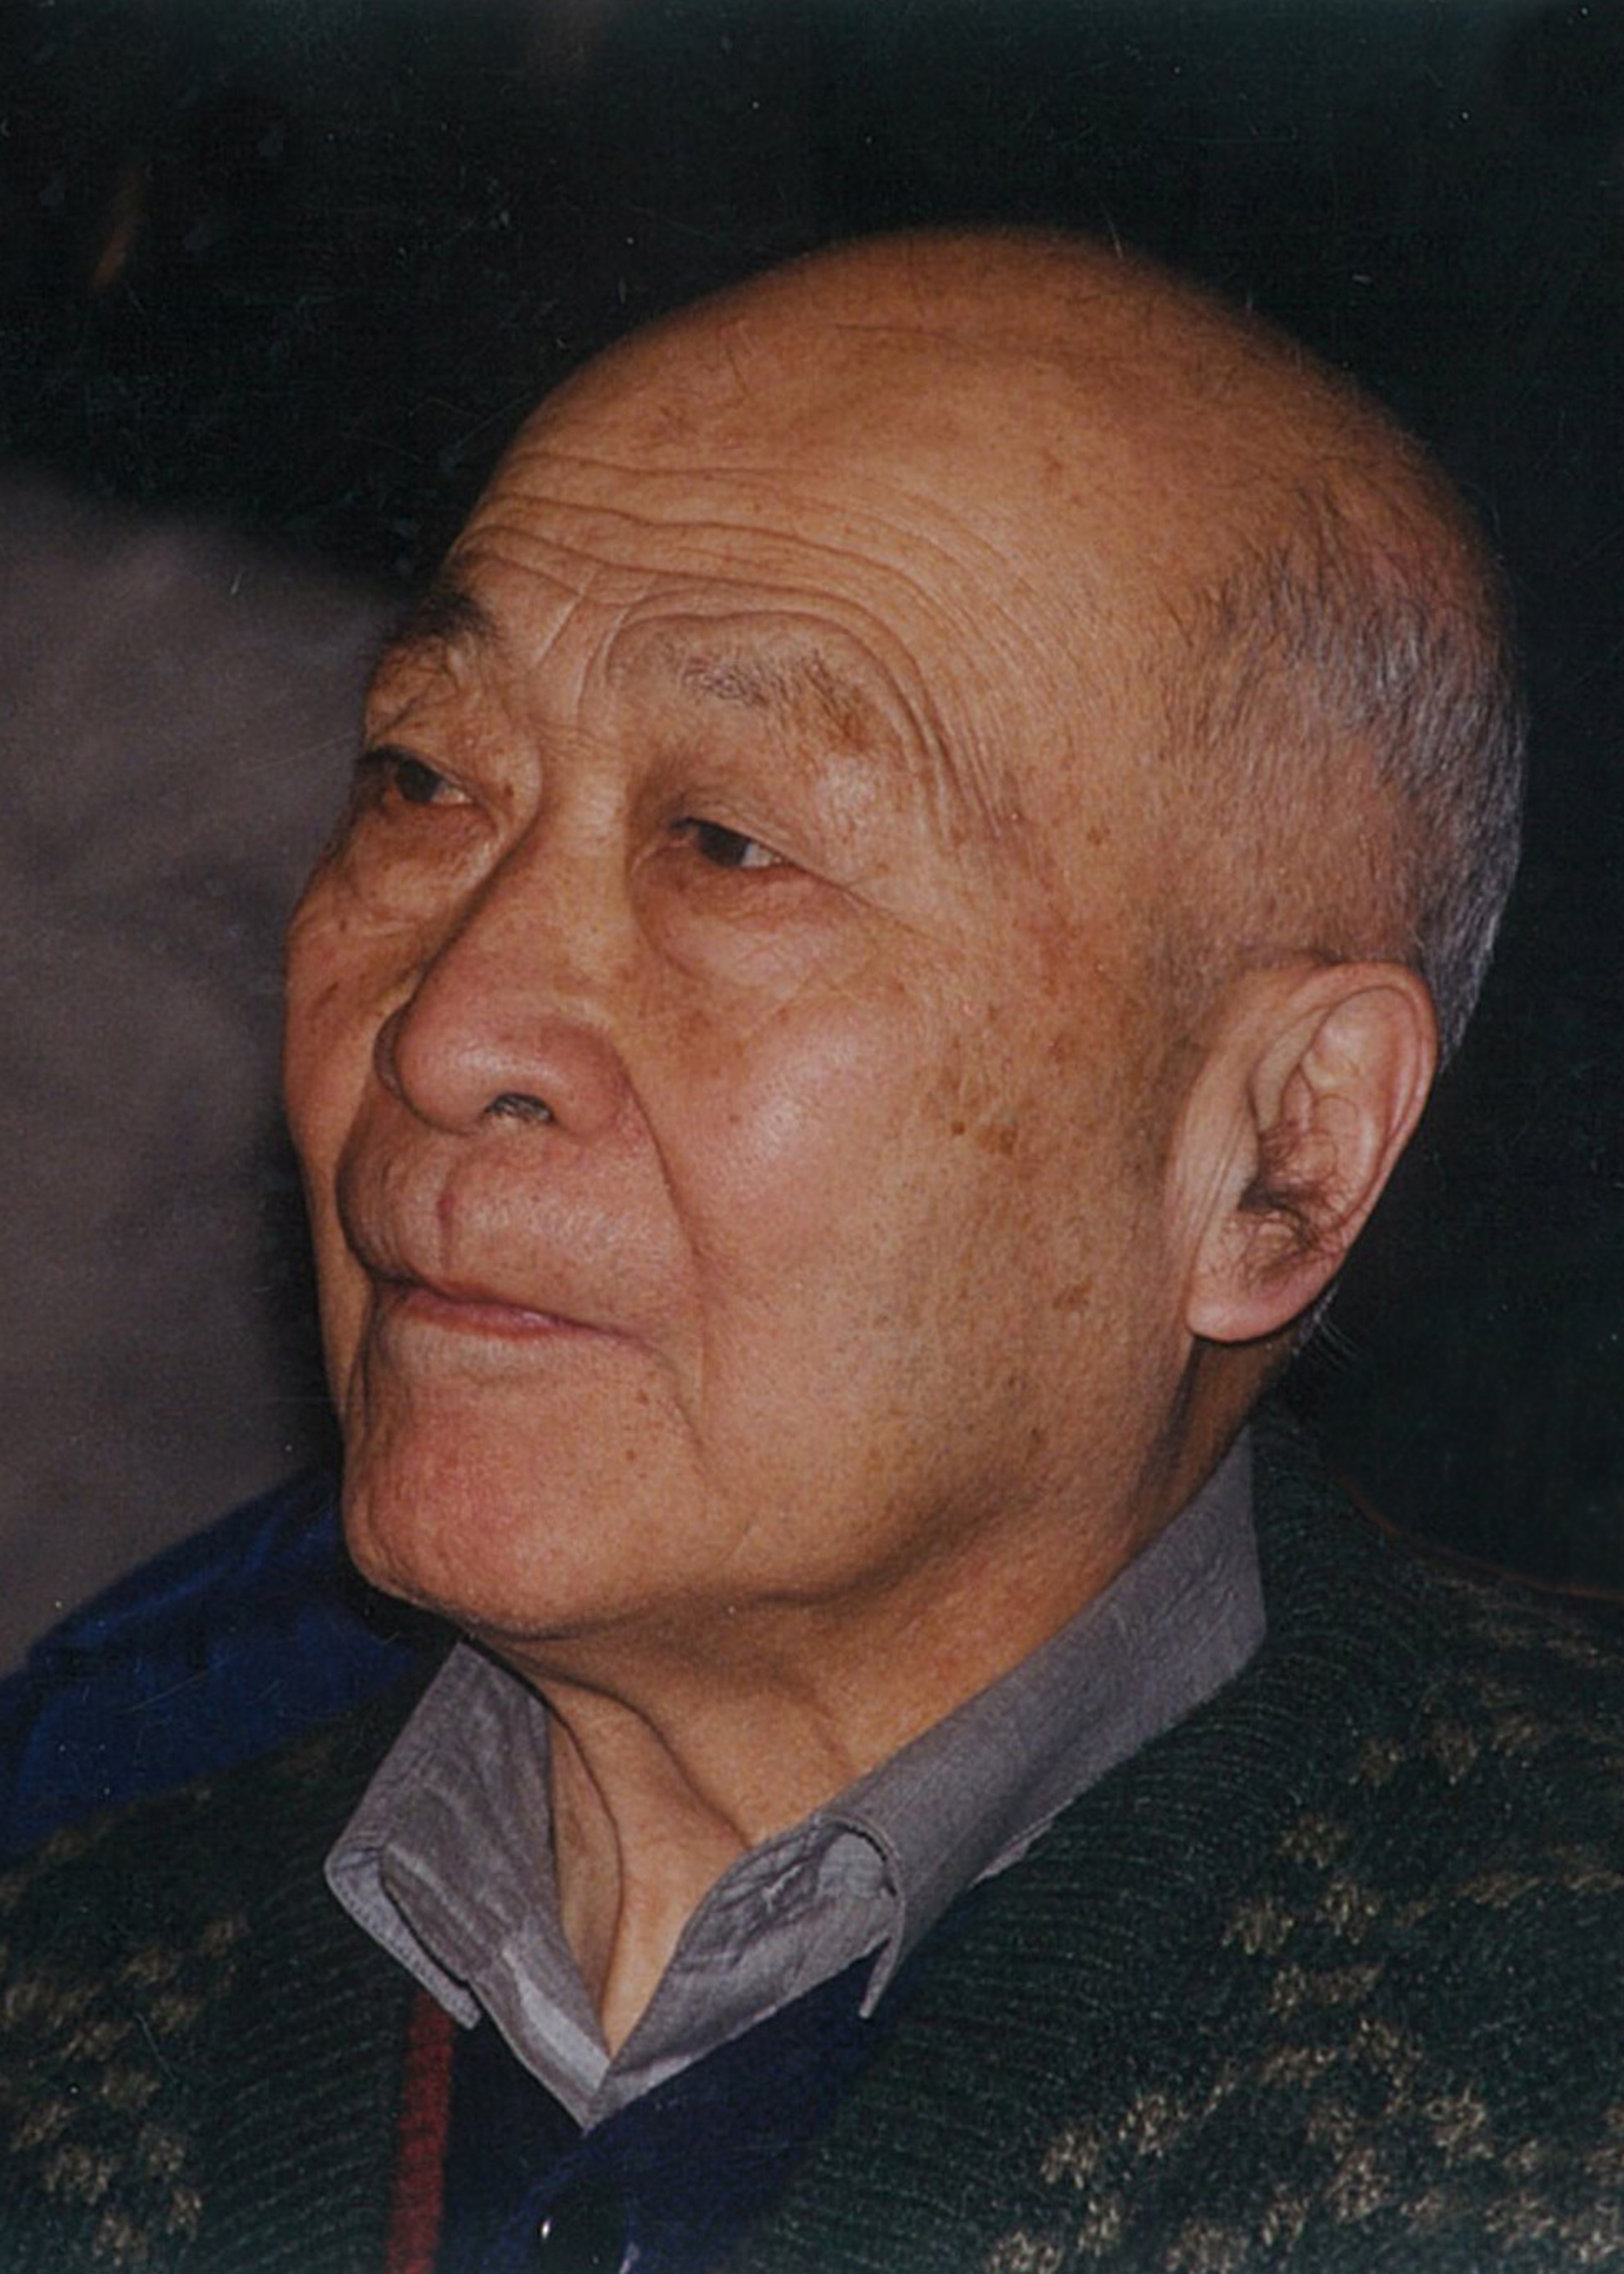
\includegraphics[height=0.64\textwidth,width=0.46\textwidth,viewport=0 0 360 520,clip]{Figures_Peking-Opera/Liu_Zengfu.jpg}
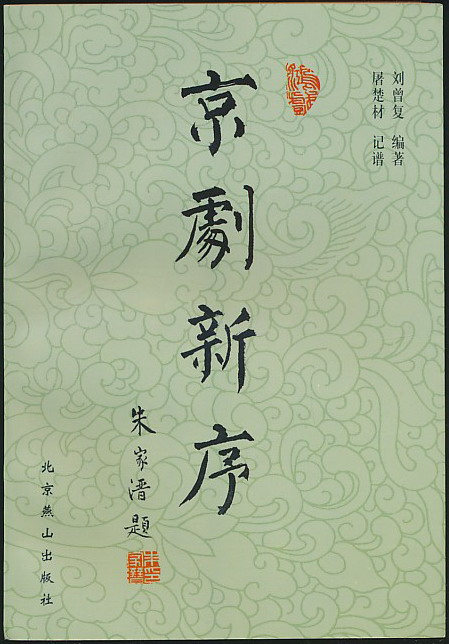
\includegraphics[height=0.58\textwidth,width=0.40\textwidth,viewport=0 0 449 644,clip]{Figures/Liu-Xinxu.jpg}
%\caption{刘曾复先生}
\label{Liu_Xinxu}
\end{figure}
}

\frame
{
	\frametitle{科学思想指导下的京剧研究:~\textcolor{red}{去伪存真}}
``系统分析''思想贯穿了刘曾复教授对京剧表演艺术研究的全过程
%总结了京剧特色和艺术风格,前者是基于对中国戏曲各剧种的音韵声腔、表演、化妆等的一般共同属性横向比较,后者则是通过解析程长庚-谭鑫培-杨(小楼)、梅(兰芳)、余(叔岩)传承中延续、完善的艺术风格后提炼的;书中
	\begin{itemize}
		\item \fontsize{8.2pt}{6.2pt}\selectfont{选择可观测、可度量的``广谱型''指标,表征京剧老生演唱和表演风格,评估由此产生的流派风格的影响}%的讨论,则是使人对谭及身后的影响一目了然;至于对。这种``多指标'' 、 ``定性-定量结合''的评价, 实际上是科研中系统研究思想在京剧研究的应用。
\begin{figure}[h!]
\centering
\vspace{-0.1in}
%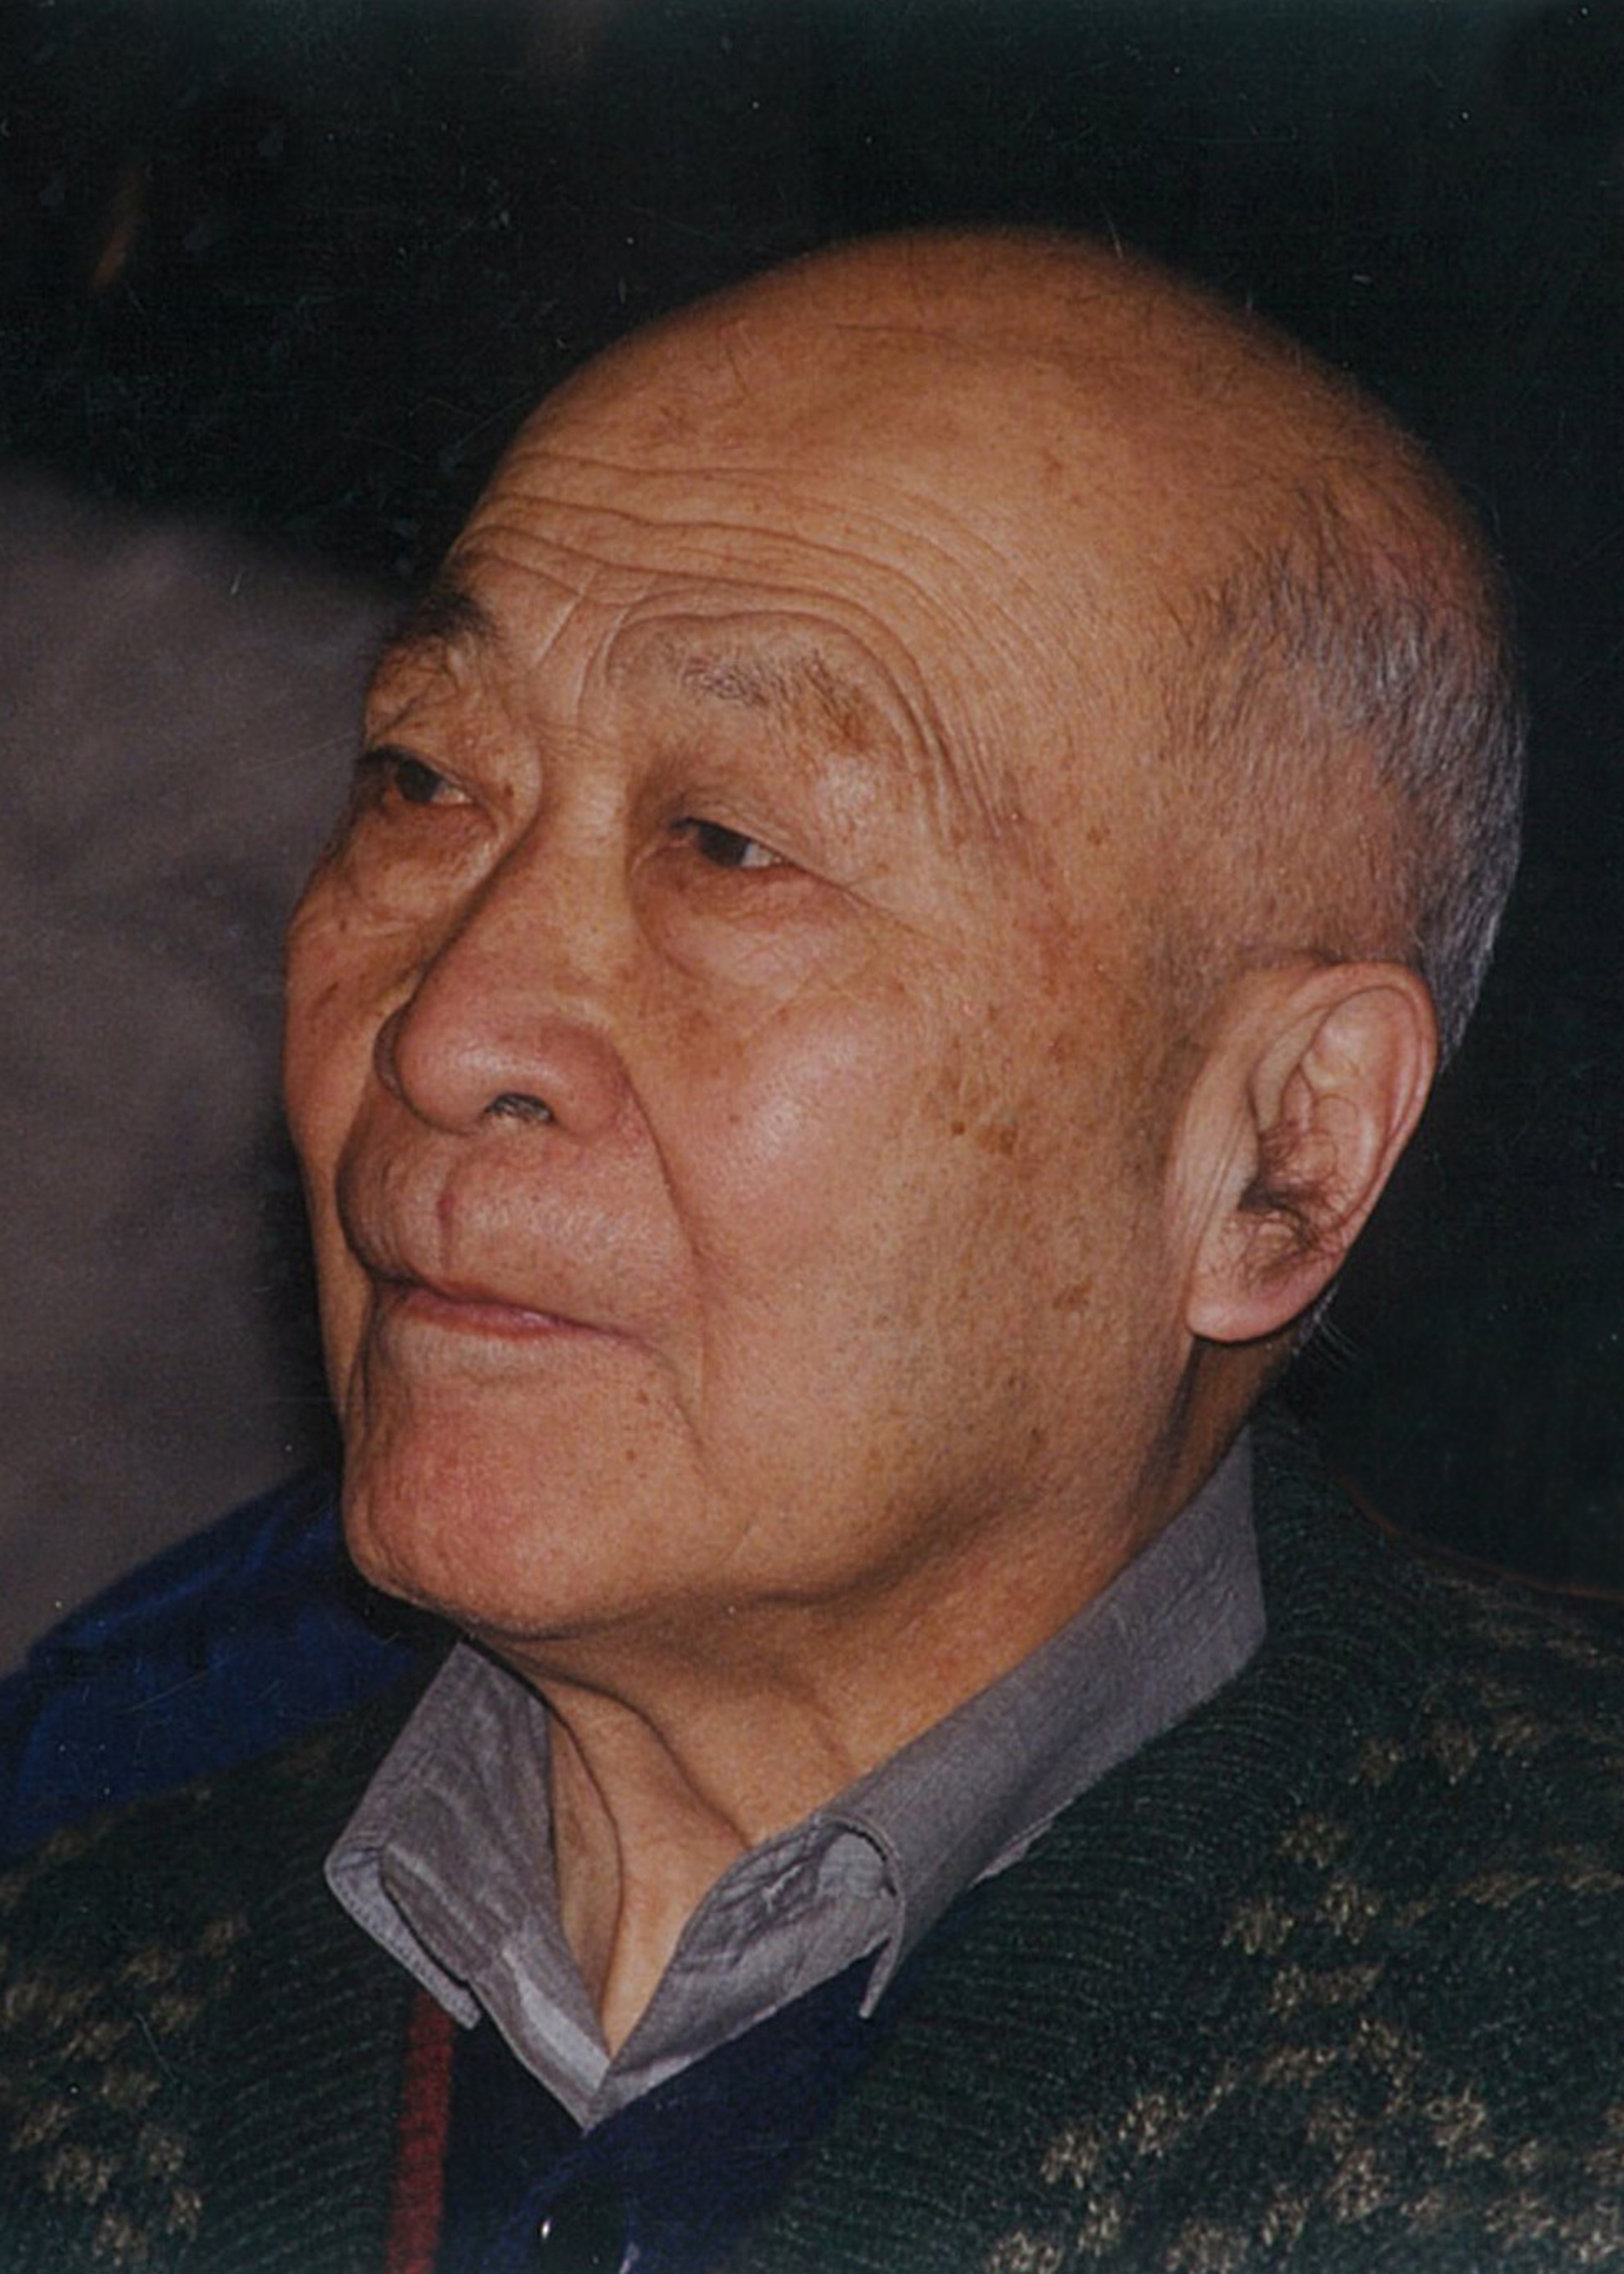
\includegraphics[height=0.64\textwidth,width=0.46\textwidth,viewport=0 0 360 520,clip]{Figures_Peking-Opera/Liu_Zengfu.jpg}
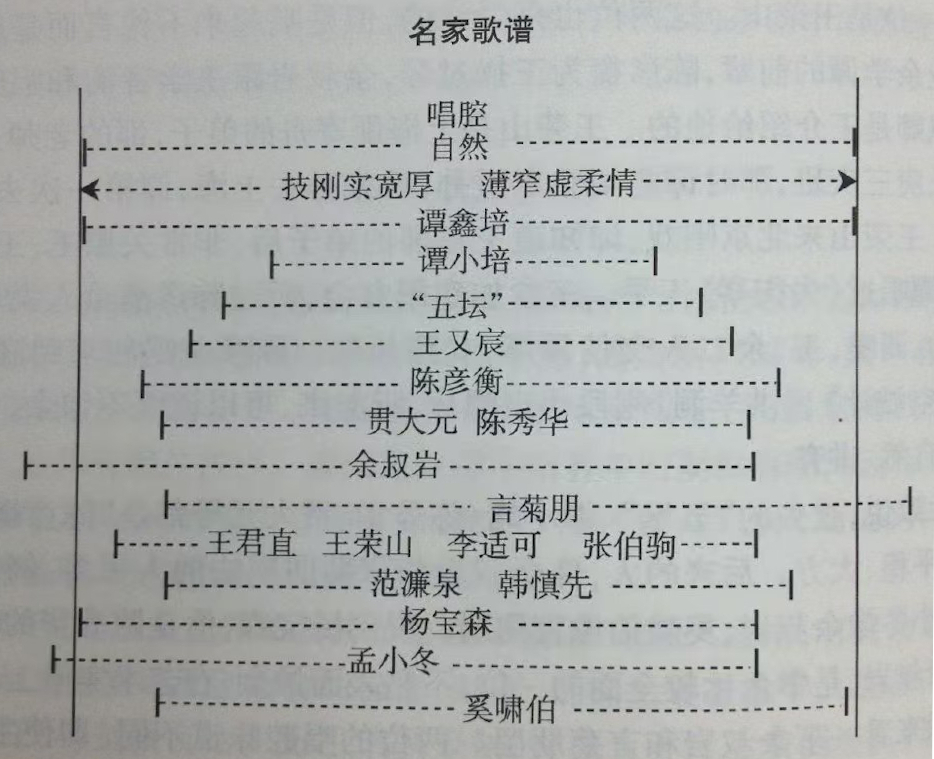
\includegraphics[height=0.40\textwidth,width=0.50\textwidth,viewport=0 0 230 185,clip]{Figures_Peking-Opera/Broad_spectrum-analysis.jpg}
%\caption{刘曾复先生}
\label{Liu_Xinxu-Analysis}
\end{figure}
\item \fontsize{8.2pt}{6.2pt}\selectfont{选择``音韵法则''、``师承''和``剧种源流''作为\textcolor{red}{特征向量},系统地梳理京剧体系中各流派、行当近百年来的传承、发展与嬗变脉络,具有一般性原则}
\item \fontsize{8.2pt}{6.2pt}\selectfont{应用系统分类的思想,研究京剧脸谱,揭示其内在逻辑,成果斐然}
	\end{itemize}
}

\frame
{
	\frametitle{科学精神}
	\begin{itemize}
		\item \textcolor{blue}{严谨专注、身体力行}\\
			对待工作:~``搞科学实验必须要有日以继夜的工作精神''\\
			\vskip 1pt
			对待爱好:~京剧通人 
		\item \textcolor{blue}{不求闻达、坚持真理}\\
			对待``针刺麻醉''研究的态度:\\
			``全国只有两个人不做‘针麻’研究,南方冯德培、北方是我''\\
			\vskip 1pt
			对传统京剧思想性的认知:\\
			``阳春''、``白雪''与``下里''、``巴人''的价值思辩
		\item \textcolor{blue}{尊师重道、谦冲自牧}\\
			介绍拉瓦锡、谢灵顿、高尔基和卡哈等伟大科学家的贡献\\
			铭记张锡钧教授、沈雋淇教授、王志均教授等师友的帮助\\
			\vskip 1pt
			留下大量京剧旧闻、掌故的口述、文字和影音资料
		\item \textcolor{blue}{奖掖后进、有教无类}
	\end{itemize}
}

\frame
{
	\frametitle{深刻的洞见}
{\fontsize{7.2pt}{4.2pt}\selectfont{今天的生理学,由于电子学和计算机科学的新发展和应用,不少生理学工作者在思想和方法上产生了``战略性''的变化,\textcolor{purple}{在工作中更合理和更有效地发挥学说和实验的作用这种工作还是处于幼稚时期,绝不是万能的,原因是许多系统的数学模型建立起来还有困难,尽管近百年来许多生理学工作都涉及到和运用了数学模型。}今后的生理学研究工作者应该放宽眼界,大展才能,站在新的基础之上,作出新的贡献。}}
\begin{figure}[h!]
\centering
\vspace{0.05in}
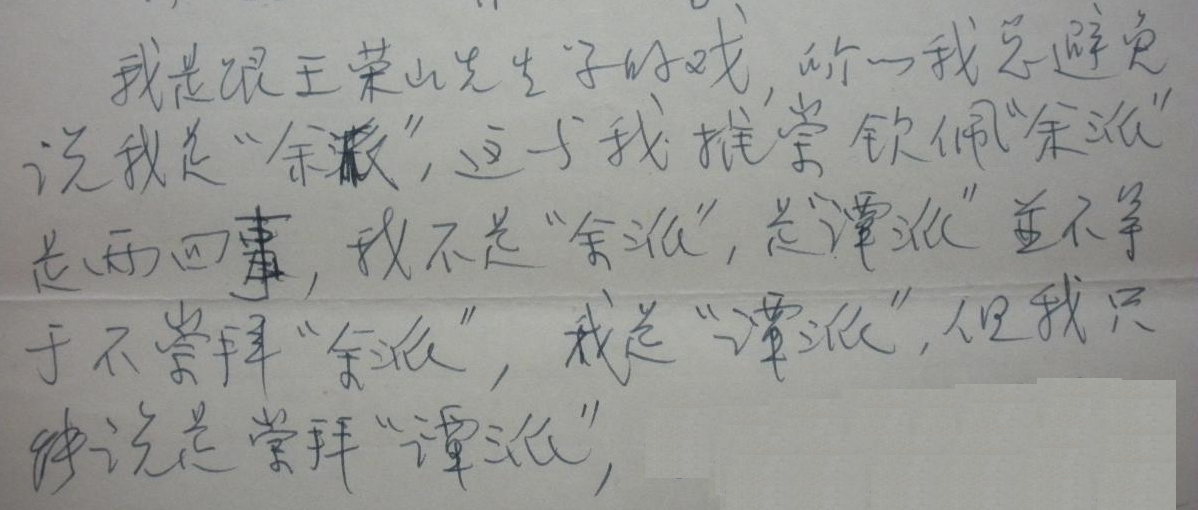
\includegraphics[height=0.45\textwidth,width=0.55\textwidth,viewport=0 0 1198 1067,clip]{Figures_Peking-Opera/Liu_Letter.jpg}
%\caption{刘曾复先生}
\label{Liu_Letter}
\end{figure}
}

\appendix
\frame
{
	\frametitle{\fontsize{20.0pt}{5.2pt}\selectfont{\textcolor{black}{~~~~~~~~~深切缅怀~刘曾复~教授}}}
\begin{figure}[ht]											      %
\centering
\vspace{-0.1in}
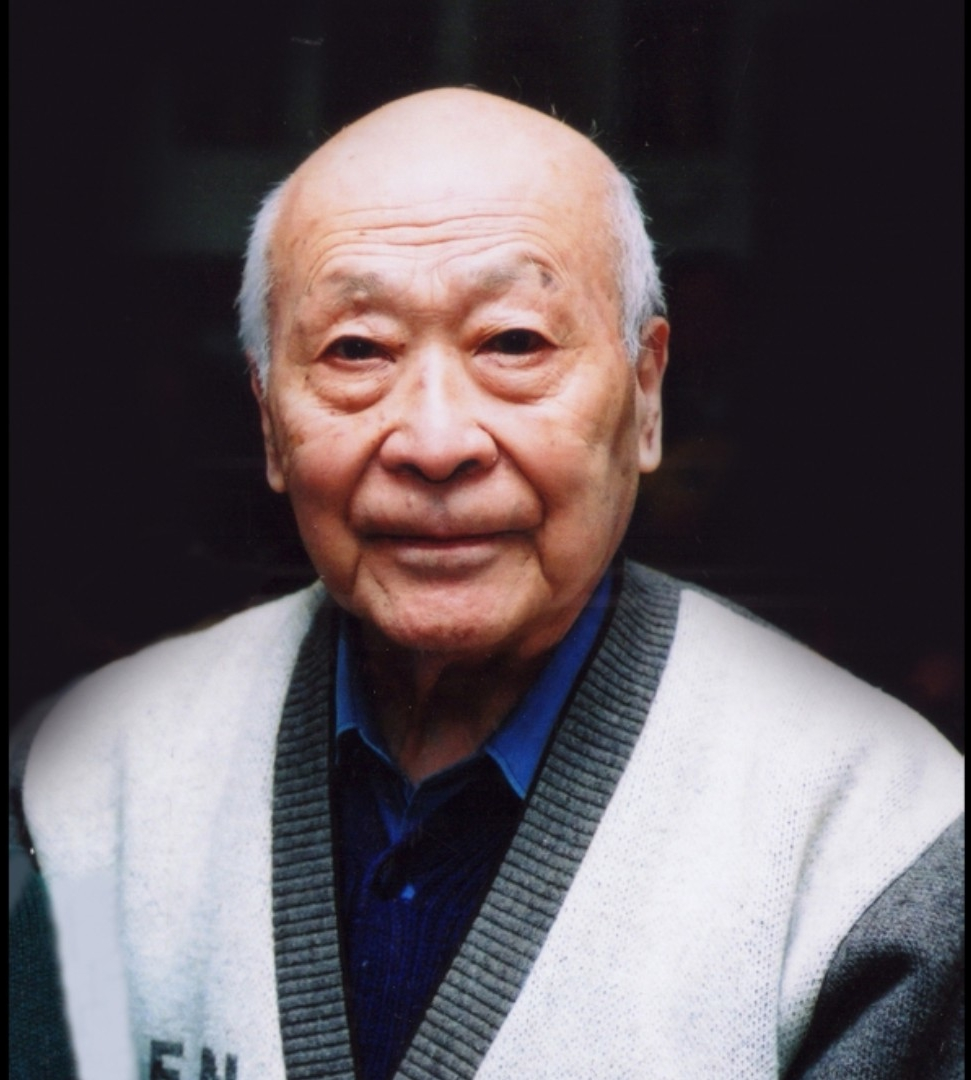
\includegraphics[height=0.60\textwidth,width=0.55\textwidth,viewport=0 0 230 260,clip]{Figures/Liu_Zengfu_2.jpg}
%	\includemovie[poster, autostart,controls, mouse, url, text=(xx), repeat] {0.8\textwidth}{0.6\textwidth}{traffic.avi}		      %
%	\includemovie[poster, controls, mouse, url] {0.8\textwidth}{0.6\textwidth}{traffic.avi}		      %
	%\includemovie[poster, controls, mouse, url] {0.8\textwidth}{0.6\textwidth}{Yuan_Kuocheng.mp4}	      %
	\includemovie[poster, controls, mouse, url] {0.8\textwidth}{0.05\textwidth}{Figures_Peking-Opera/Liu-Xiongzhouguan.mp3}     %
	\includemovie[poster, controls, mouse, url] {0.8\textwidth}{0.05\textwidth}{Figures_Peking-Opera/Liu-Pantaohui.mp3}	      %
\caption{刘曾复教授京剧遗馨}											      %
\end{figure}												      %
%\caption{刘曾复先生}
}
%\frame
%{
%	\frametitle{答辩合影}
%\begin{figure}[h!]
%\centering
%\vspace{-10.5pt}
%\includegraphics[height=0.62\textwidth,width=0.9\textwidth,viewport=0 0 820 600,clip]{Figures_Peking-Opera/Thesis_Defense_2007.jpg}
%\caption{\textrm{2007.12.15博士论文答辩后留影:}\\{\fontsize{7.1pt}{3.9pt}\selectfont\textrm{左起:~刘文剑教授、黄元河教授、刘若庄教授、答辩人、徐光宪教授、王德民教授、黎乐民教授}}}
%\label{Thesis_Defense_2007}
%\end{figure}
%}

%------------------------------------------------------------------------Reference----------------------------------------------------------------------------------------------
		\frame[allowframebreaks]
{
\frametitle{其他参考文献}
\begin{thebibliography}{99}
{\tiny
	\bibitem{Shengli_Shuoyuan}{杜金香~主编~《生理说苑——刘曾复论文选编及其他》~ 首都医科大学~(内部刊印) (2002)}
	\bibitem{Jingju_Shuoyuan}{刘曾复~著、《京剧说苑》(封杰~主编~``国粹传承\!$\cdot$\!京剧研究丛书'')~ 学苑出版社~(北京)~(2012)}
	\bibitem{Liuzengfu_Wencun}{刘曾复~著、娄悦~编~《刘曾复京剧文存》~ 学苑出版社~(北京)~(2013)}
}
\end{thebibliography}
%\nocite*{}
}
%\frame
%{
%	\frametitle{说戏剧本集}
%\begin{figure}[h!]
%\centering
%\vspace{-10.5pt}
%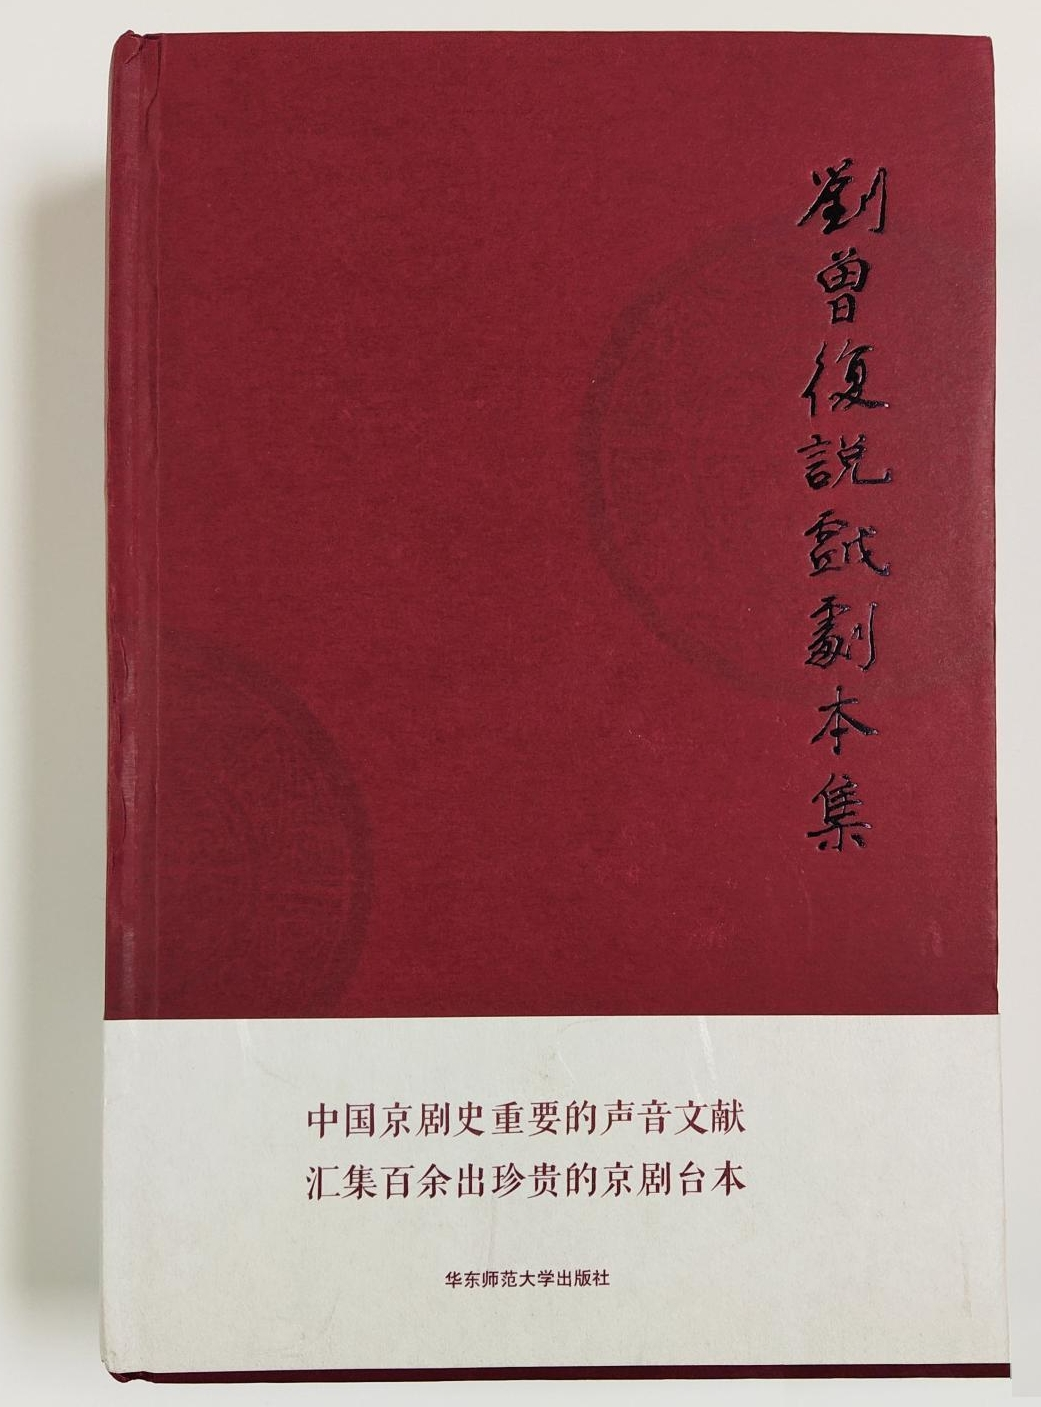
\includegraphics[height=0.68\textwidth,width=0.49\textwidth,viewport=0 0 1030 1400,clip]{Figures_Peking-Opera/Liu_script.jpg}
%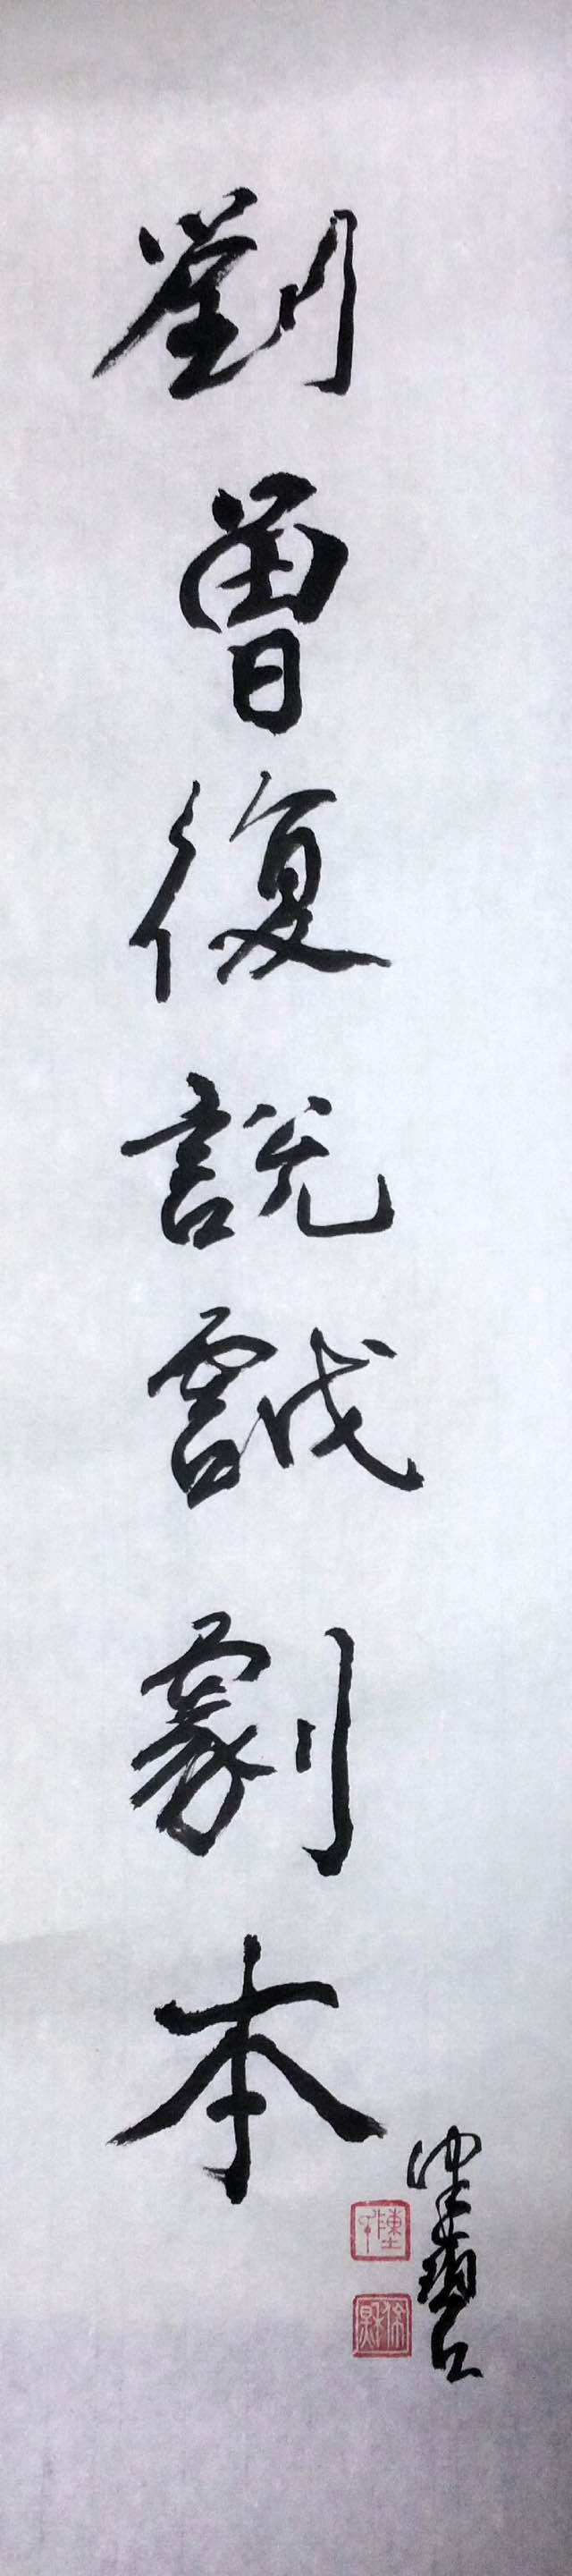
\includegraphics[height=0.68\textwidth,width=0.125\textwidth,viewport=0 0 620 2850,clip]{Figures_Peking-Opera/Liu_script-Inscription.JPG}
%\caption{\fontsize{6.1pt}{3.9pt}\selectfont\textrm{《刘曾复说戏剧本集》~陈佩秋题签~~华东师范大学出版社~(2015.08)}}
%\label{Peking_Opera_Script-2015}
%\end{figure}
%}

%\frame
%{
%	\frametitle{京剧唱腔选}
%\begin{figure}[h!]
%\centering
%\vspace{-10.5pt}
%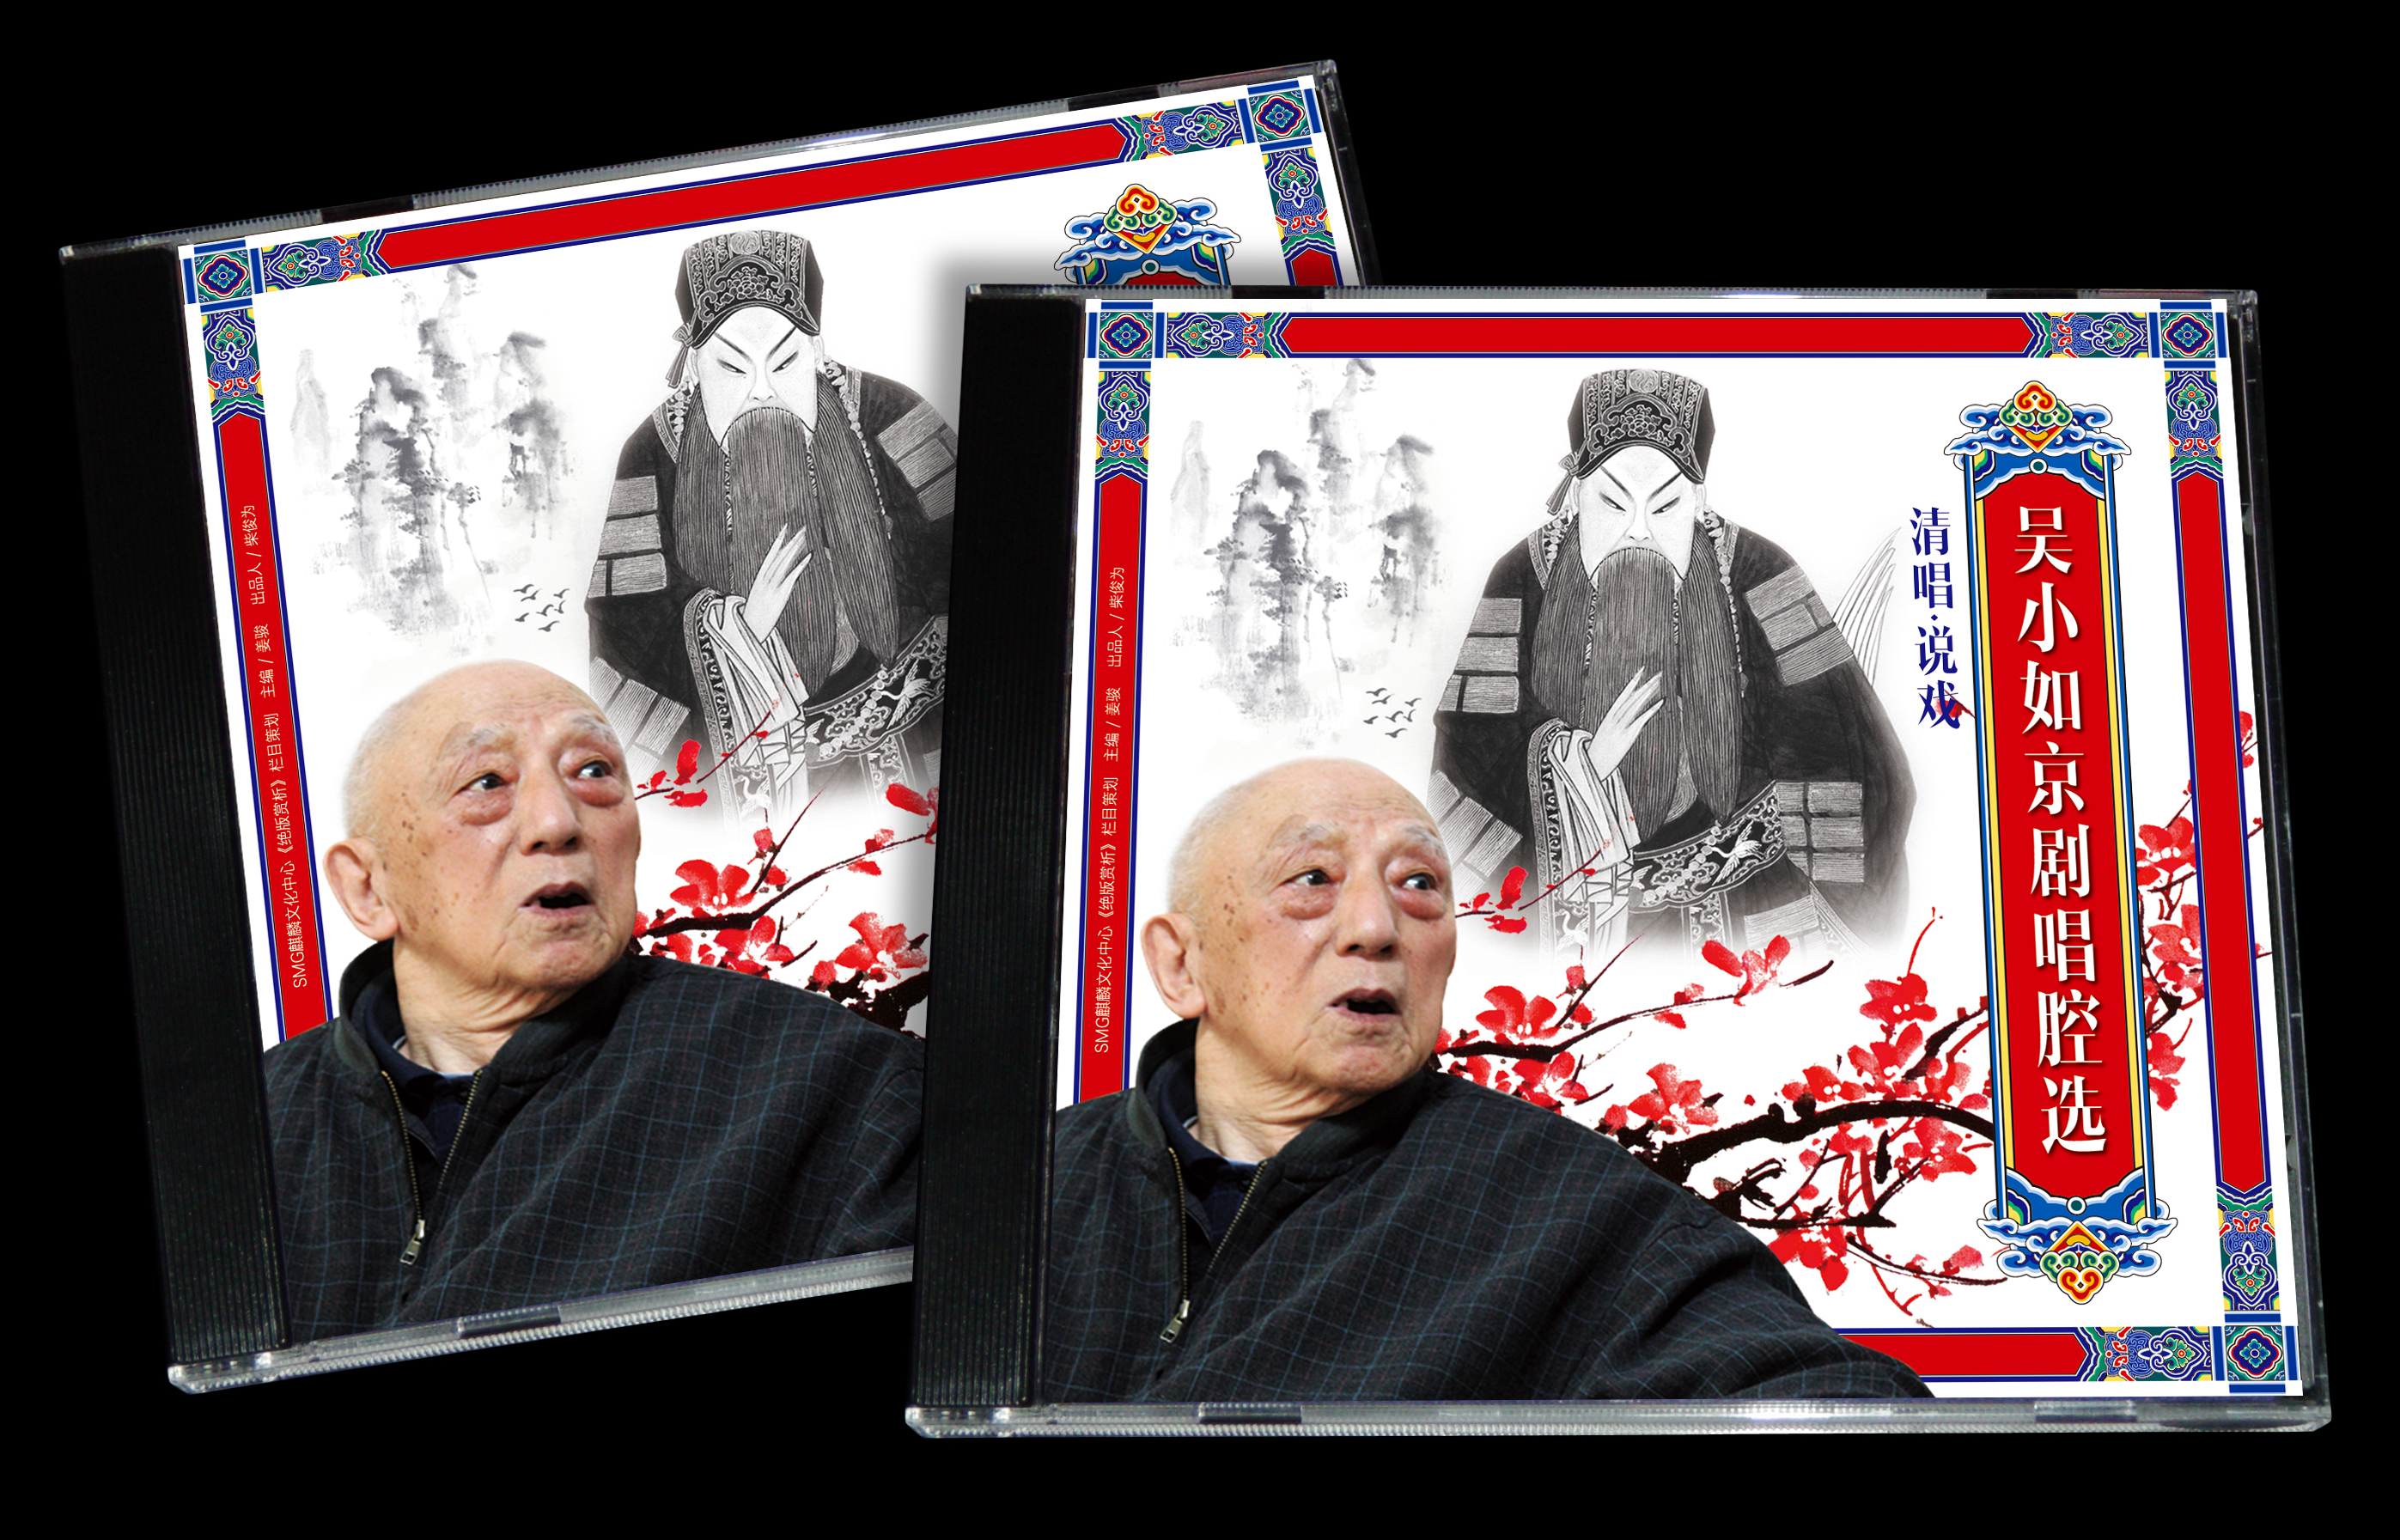
\includegraphics[height=0.65\textwidth,width=0.95\textwidth,viewport=0 0 680 450,clip]{Figures_Peking-Opera/Wu_CD.jpg}
%\caption{\fontsize{6.1pt}{3.9pt}\selectfont\textrm{《吴小如京剧唱腔选》~绝版赏析栏目组~~新汇集团上海音像有限公司~(2013.03)}}
%\label{Peking_Opera_CD-2012}
%\end{figure}
%}

%\begin{frame}
%	\frametitle{frame with sound}
%\dots
%\includemedia[ 
%	label=my_sound,
%	width=1ex, height=1ex, 
%	transparent,
%	activate=pageopen, 
%	deactivate=onclick,
%	addresource=Figures_Peking-Opera/Liu-Xiongzhouguan.mp3,
%	flashvars={source=Figures_Peking-Opera/Liu-Xiongzhouguan.mp3
%                  &autoPlay=true
%                  &loop=true
%                  &hideBar=false}
%	  ]{}{APlayer.swf}
%\dots
%\end{frame}

%\begin{frame}{other frame}
%\dots
%\end{frame}

%\pdfpageattr{/AA <</O <</S/JavaScript/JS (annotRM['my_sound'].activated=false;)>> >>}
%\begin{frame}{frame where sound stops}
%\dots
%\end{frame}

%\begin{frame}{another dumb frame}
%\dots
%\end{frame}

%%%%%%%%%%%%%%%%%%%%%%%%%%%%%%%%%%%%%%%%%%%%%%%%%%%%%%%%%%%%%%%%%%%%%%%%%%%%%%%%%%%%%%%%%%%%%%%%%%%%%%%%%%%%%%%

%\frame<handout:0>
%{
%	\frametitle{}
%\begin{figure}[h!]
%\centering
%\animategraphics[autoplay, loop, height=2.0in]{1}{Figures_Peking-Opera/vlcsnap-}{01}{10}
%\label{Pro_Liu_gif}
%\end{figure}
%}

%%%%%%%%%%%%%%%%%%%%%%%%%%%%%%%%%%%%%%%%%%%%%%%%%%%%%%%%%%%%%%%%%%%%%%%%%%%%%%%%%%%%%%%%%%%%%%%%%%%%%%%%%%%%%%%

%------------------------------------------------------------------------Reference----------------------------------------------------------------------------------------------
%\begin{thebibliography}{99}
%-----------------------------------------------------------------------------------------------------------------------------------------------------------------------%
%\frame
%{
%\frametitle{主要参考文献}
%{\small
%\bibitem{Singh_Book}\textrm{D. J. Singh. \textit{Plane Wave, PseudoPotential and the LAPW method} (Kluwer Academic, Boston,USA, 1994)}					%
%  \nocite{*}																				%
%}
%}
%\end{thebibliography}
%\frame%[allowframebreaks]
%{
%\begin{thebibliography}{99}
%\frametitle{主要参考文献}
%{\small
%	\bibitem{Zhu_Tuishilu}朱家溍 著, {\textit{故宫退食录}}\;\textrm{({\textit{上、下}})}\:北京出版社, 北京, 1999\\
%朱家溍 著, {\textit{故宫退食录}}\;\textrm{({\textit{上、下}})}\:紫禁城出版社, 北京, 2009
%	\bibitem{Liu_Xinxu}刘曾复 编著、屠楚材 记谱, {\textit{京剧新序}}\:燕山出版社, 北京, 1999\\
%{\fontsize{7.0pt}{3.9pt}\selectfont 刘曾复 编著、屠楚材 记谱,娄悦、何毅 整理, {\textit{京剧新序}}\;\textrm{(修订版)}\:学苑出版社, 北京, 2009}\\
%刘曾复 传述, {\textit{刘曾复说戏剧本集}}\:华东师范大学出版社, 上海, 2015
%	\bibitem{Wu_Wenlu}吴小如 著, {\textit{吴小如戏曲文录}}\:北京大学出版社, 北京, 1995 \\
%	吴小如 著, {\textit{吴小如戏曲随笔集补编}}\:天津古籍出版社, 天津, 2006
%	\bibitem{XQYS1-32_1983}\textrm{刘曾复、王世续、王金彦, 京剧老生把子见闻录\:\textit{戏曲艺术}, \textbf{第一期} (1983), 32}
%	\bibitem{ZGXJ1-57_1993}\textrm{刘曾复, 京剧书文指伪录\:\textit{中国戏剧}, \textbf{第01期} (1993), 57}
%}
%\nocite*{}
%\end{thebibliography} 
%}

%-----------------------------------------------------------Beamer下不建议使用bib,因为涉及分页--------------------------------------------------------------------------%
